
\documentclass[conference]{IEEEtran}

\usepackage{float} 
\usepackage{url}  
\usepackage{multirow}
\usepackage{subcaption}
\usepackage{booktabs}
\usepackage{cite}
\pagestyle{plain}
\usepackage{amsmath}
\usepackage{float}
\usepackage{tikz}
\usetikzlibrary{shapes.geometric, arrows, positioning}
\usepackage{placeins}


\ifCLASSINFOpdf
  \usepackage[pdftex]{graphicx}
\fi

\hyphenation{op-tical net-works semi-conduc-tor}

\begin{document}


\title{Recommender Systems: Implementation of Collaborative Filtering Algorithms and Benchmark}

\author{\IEEEauthorblockN{\\ Hugo Veríssimo}
\IEEEauthorblockA{Foundations of Machine Learning 24/25\\
University of Aveiro\\
Aveiro, Portugal\\
hugoverissimo@ua.pt}
\and
\IEEEauthorblockN{\\ João Cardoso}
\IEEEauthorblockA{Foundations of Machine Learning 24/25\\
University of Aveiro\\
Aveiro, Portugal\\
joaopcardoso@ua.pt}}

\maketitle
\thispagestyle{plain}

\begin{abstract}
Recommender systems have been used reliably since their early inception the 90's, and the field exploded upon the introduction of the Netflix prize, which aimed at developing the best and most efficient recommender system for their movie platform. In this work three recommender systems based on collaborative filtering are developed and presented, based on one of the MovieLens datasets. The models are compared considering their error metrics, and the capacity to rank items accurately. The models are compared with the literature, focusing on the framework used for comparison. 
\end{abstract}

\begin{quote}
\small
\noindent
\textbf{Keywords:} MovieLens, GroupLens, Recommender System, Collaborative Filtering, Linear Regression, FunkSVD
\end{quote}

\IEEEpeerreviewmaketitle


\section{Introduction}

Since the early 90's that the production rate of multimedia content has increased dramatically (pun intended). Initially, users relied mostly on video store owners, film critics on newspapers, friends. With increasing volumes of content, recommender systems have appeared as data-driven methods to reliably and quickly recommend movies based on the users' own appreciations.

% The use of similar datasets can help facilitate the comparison of RS, but it isn't the only way. Maybe add this further down the document, it is not so relevant in the introduction.

Recommender systems are information tools that provide users with recommended items (ideally) based on their list of preferences \cite{Konstan2012,KATARYA2017105}. These can be divided in different types, depending on the algorithm and approach to the data. Three categories can be considered: non-personalized, content-based, and collaborative filtering algorithms. Regardless of the algorithm of choice, these face crucial challenges: cold start problem (where it is difficult to tailor recommendations to a user without known preferences, or recommend an item with no reviews); data sparsity (given that most users review few items in the universe of possible items, leaving most of the user/item matrix empty); and scalability (as data grows exponentially, processing becomes evermore expensive and troublesome). These systems have been widely used in many different areas (online shopping, music, books, movie recommendation), and significant investment has gone into developing evermore personalized algorithms. A notable case for this was the Netflix prize competition in 2009, a moment where the research in the field skyrocketed. As a result, many algorithms fitted and tested on different conditions and datasets have been developed. With this came the need to develop better frameworks for comparison, considering not only the metrics, but data preprocessing, preparation, and routine, in order to ensure reproducibility across models and authors \cite{10.1145/2645710.2645746}.

For that reason, the developed recommender systems is based on one of the most widely used movie databases, MovieLens dataset, for education and development \cite{Harper2015}. The choice of this dataset allowed for a based comparison with algorithms from the literature, and facilitate the analysis and interpretation of the results here presented. 

\section{State of the Art}

The field of recommender systems is wide and covers many different algorithms and techniques. In this paper we focus on collaborative filtering using matrix factorization, as it is the main focus of the work here developed.

The Netflix prize is often cited as one of the main drivers for research in collaborative filtering recommender systems \cite{netflix_prize_2009}. One of the initial awarded proposals was that by Brandyn Webb, known by his alias "Simon Funk". Despite the name of the algorithm (FunkSVD), Singular Value Decomposition is not used, it uses instead gradient descent to find the latent feature values used to predict the ratings matrix. The algorithm uses only the available ratings, representing a great advantage against SVD methods that struggle with mostly sparse matrices. 

Unlike SVD, the original matrix is decomposed between two matrices (for users and movies), where the diagonal matrix typically found in SVD is merged into one of the two. Since the original matrix is so sparse, the \textit{u} matrix and the \textit{v} matrices are initiated randomly, and estimated by minimizing the error relative to the original matrix via gradient descent.

\begin{equation}
r_{ij} = u_i \cdot v_j
\end{equation}
\begin{align}
u_{if}(\text{new}) &= u_{if}(\text{old}) + 2\alpha(r_{ij} - \tilde{r}_{ij})v_{jf} \\
v_{jf}(\text{new}) &= v_{jf}(\text{old}) + 2\alpha(r_{ij} - \tilde{r}_{ij})u_{if}
\end{align}

There is a caveat however, given that the model requires fine tuning of numerous parameters (number of latent features, learning rate, training iterations, regularization parameter), which can lead to overfitting \cite{Funk2006}. 

In the work by Zhou et al., alternating least squares with weighted  $\lambda$ regularization (ALS-WR). 
\begin{align}
f(U, M) &= \sum_{\{i, j\} | r_{i,j} \in I} \left( r_{i,j} - u_i^T m_j \right)^2 \nonumber \\
&\quad + \lambda \left( \sum_i n_{u_i} \| u_i \|^2 + \sum_j n_{m_j} \| m_j \|^2 \right)
\end{align}

The algorithm expresses the rating matrix as the product of two smaller matrices U (user matrix) and M (item matrix). Thanks to its simplicity, the algorithm tackles both scalability and sparseness of user profiles, with the added bonus of not overfitting \cite{10.1007/978-3-540-68880-8_32}. 

A third model by Gopalan et al. uses a probabilistic approach by assuming that the observed rating is drawn from a Poisson distribution, which is parameterized by the inner product of a user weights vector and an item weights vector.

\begin{equation}
y_{ui} \sim Poisson(\theta_u^T \beta_i)
\end{equation}
\noindent
Where:
\begin{itemize}
    \renewcommand{\labelitemi}{~}
    \item \textit{User weights:} $\theta_u = [\theta_{u1}, \dots, \theta_{uk}]$
    \item \textit{Item weights:} $\beta_i = [\beta_{i1}, \dots, \beta_{ik}]$
    \item $\theta_{uk} \sim Gamma(a, b)$
    \item $\beta_{ik} \sim Gamma(c, d)$
\end{itemize}

With this, the model is able to compute the probability for each unconsumed item that the user might enjoy \cite{gopalan2014scalablerecommendationpoissonfactorization}.

\section{Methodology}

\subsection{Data description}

The dataset MovieLens for Education and Research (small) was used to test the different models. It contains 100.836 ratings, from 0.5 to 5, for 9724 movies (and its genres) and 610 users, where each user rated at least 20 movies \cite{MovieLens}.

\subsection{Data splitting \& models implemented}

The dataset was split between train and test (80/20), which resulted in 80668 ratings for the training and 20168 for the testing dataset. Three models were developed, as described in the Table \ref{models_cf}.

\begin{table}[H]
\centering
\caption{Implemented models description.}
\label{models_cf}
\resizebox{\columnwidth}{!}{
\begin{tabular}{lc}
\toprule
\textbf{Model - features} & \textbf{Description} \\
\midrule
Model 01 - Users and Movies & Collaborative Filtering, && Linear Regression (CF-LR) \\[1em]
Model 02 - Users and Movies + Genres & Hybrid: Content-Based + Collaborative, && Linear Regression (CB-LR) \\[1em]
Model 03 - Users and Movies & Collaborative Filtering, && FunkSVD (CF-FunkSVD) \\[1em] 
\bottomrule
\end{tabular}
}
\end{table}

The models were fitted with an 8-fold cross validation to find the best hyperparameters for the considered interval. For CF-FunkSVD, the package \textit{surprise} and the tools therein \cite{surprise} were used. 

The primary error metrics employed in this study were the mean absolute error (MAE) and the root mean squared error (RMSE). The MAE considers all error equally, regardless of their size, whereas RMSE strongly penalizes larger errors.

\begin{equation}
MAE = \frac{1}{n}\sum^n_{i=1}|y_i-\hat{y}_i|
\end{equation}

\begin{equation}
RMSE = \sqrt{\frac{1}{n}\sum^{n}_{i=1}(y_i - \hat{y}_i)^2}
\end{equation}

\subsection{Exploratory data analysis}

The dataset comprises a diverse selection of movies spanning a wide range of genres, as illustrated in Fig. \ref{fig:genre_distribution}, with a total of 20 genres.

\begin{figure}[H]
    \centering
    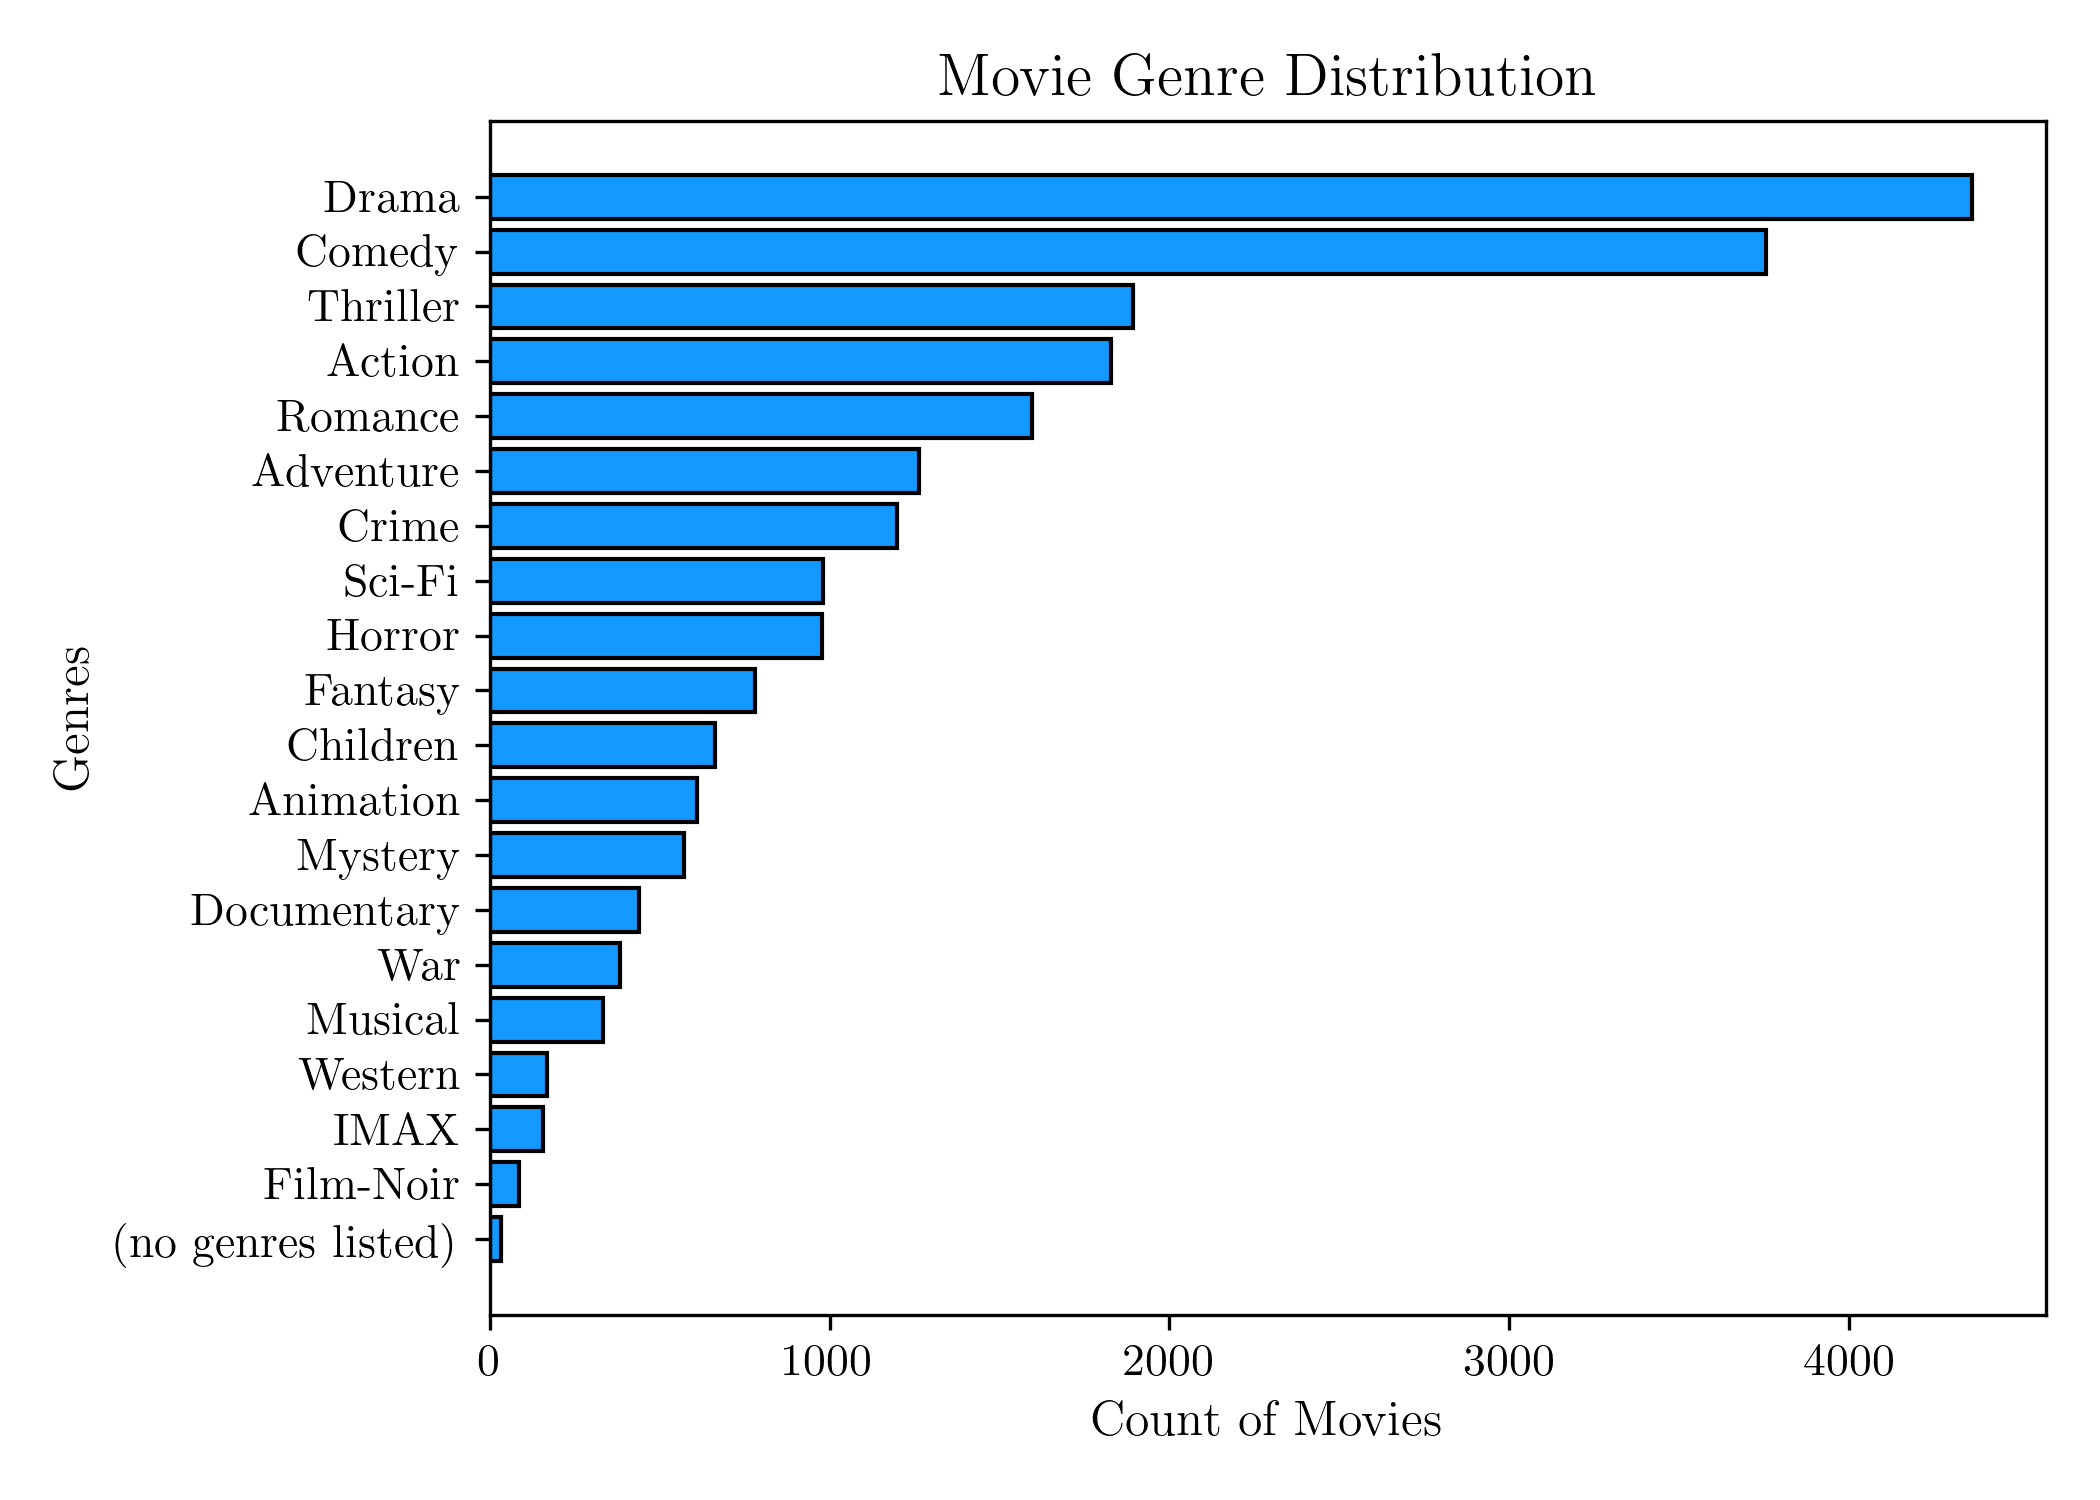
\includegraphics[width=1\linewidth]{assets/genre_distribution.png}
    \caption{Distribution of movies per movie genre.}
    \label{fig:genre_distribution}
\end{figure}

Despite the variety in genres, it's important to retain that generally movies are more complex than representing a single genre. In that sense, it is useful to assess the similarity between genres (using the cosine similarity index), as illustrated in Fig. \ref{fig:genre_similarity}. This helps understand how the task of recommending a movie can start to grow more complex as we add more and more detail to the dataset. In Table \ref{tab:genre_similarity} the five most related genres are shown.

\begin{figure}[H]
    \centering
    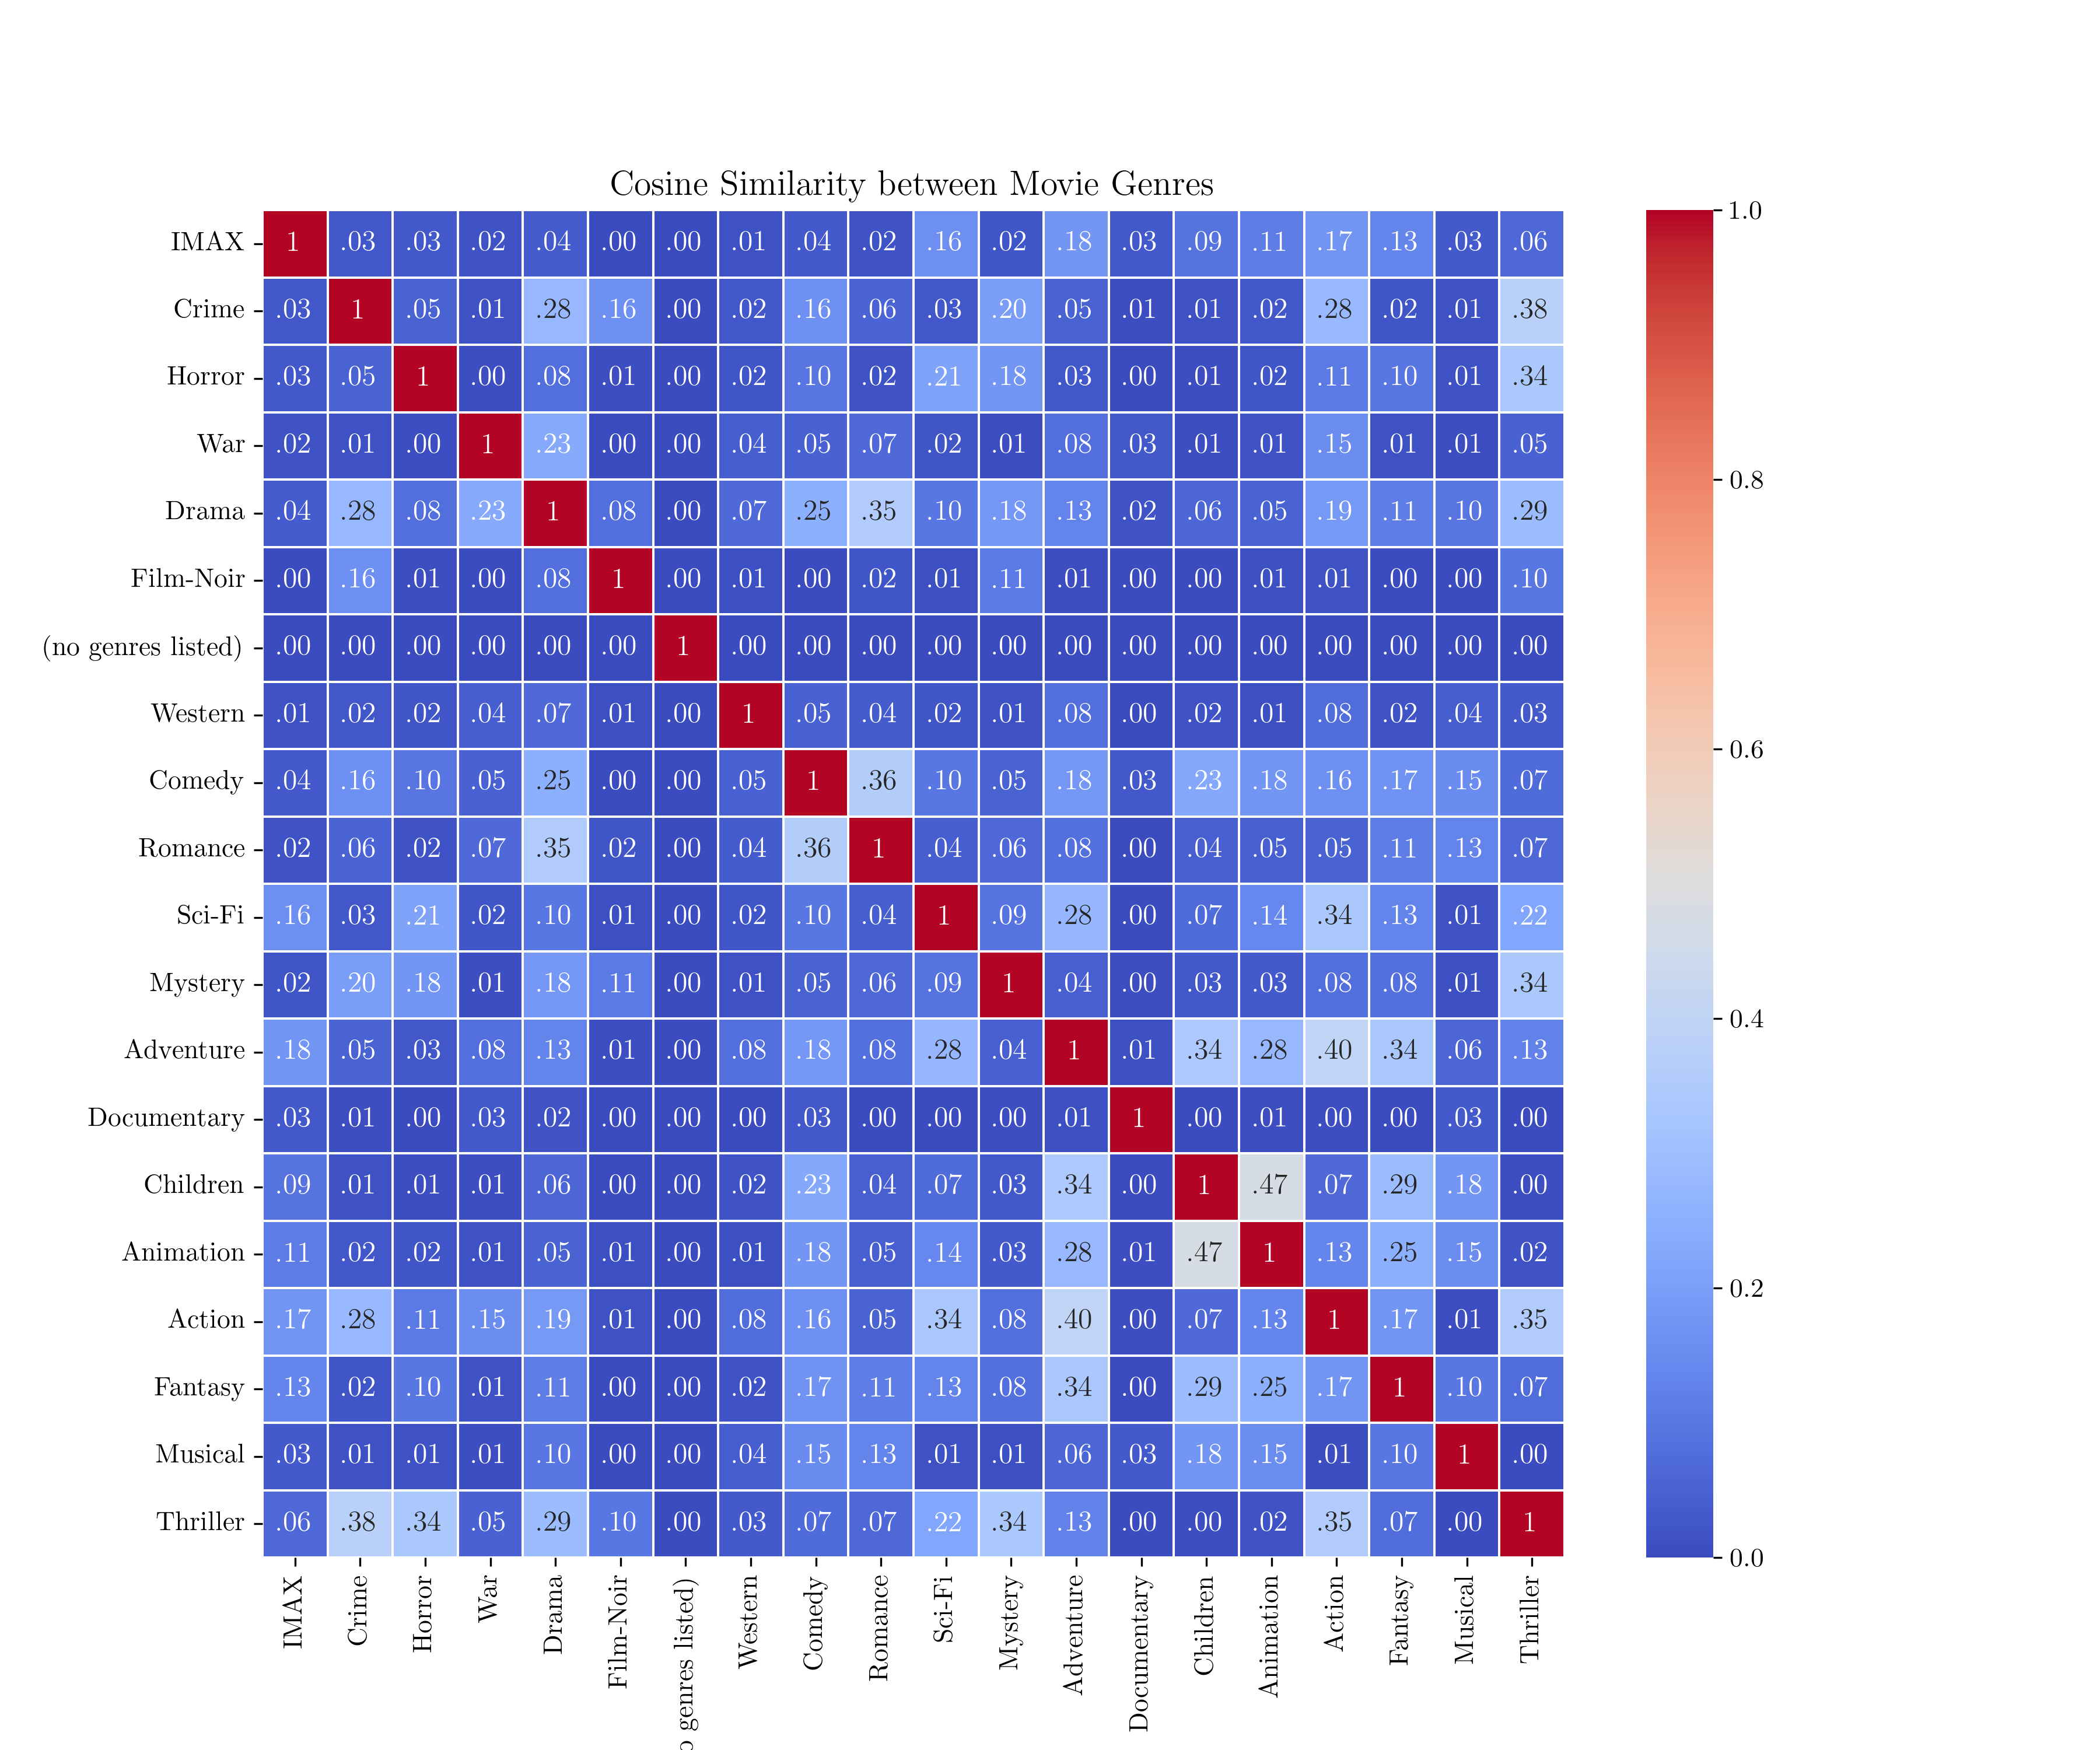
\includegraphics[width=1\linewidth]{assets/genre_similarity.png}
    \caption{Cosine similarity index between genres.}
    \label{fig:genre_similarity}
\end{figure}

\begin{table}[H]
\centering
\caption{The five most related genres per cosine similarity index.}
\label{tab:genre_similarity}
\begin{tabular}{ccr}
\toprule
\multicolumn{2}{c}{\textbf{Genres}} & \textbf{Similarity Index} \\
\midrule
Animation & Children & .47 \\ 
Action & Adventure & .40 \\
Crime & Thriller & .38 \\
Romance & Comedy & .36 \\
Romance & Drama & .35 \\
\bottomrule
\end{tabular}
\end{table} 

The dataset is relatively recent, with movies from the 2010's, going all the way back to the early 1900's, as per Fig. \ref{fig:year_distribution}. As expected, there are much fewer ratings for older movies, for two main reasons: older movies are less popular, and there are less movies in general, as movie production picked up substantially throughout the twentieth century.

\begin{figure}[H]
    \centering
    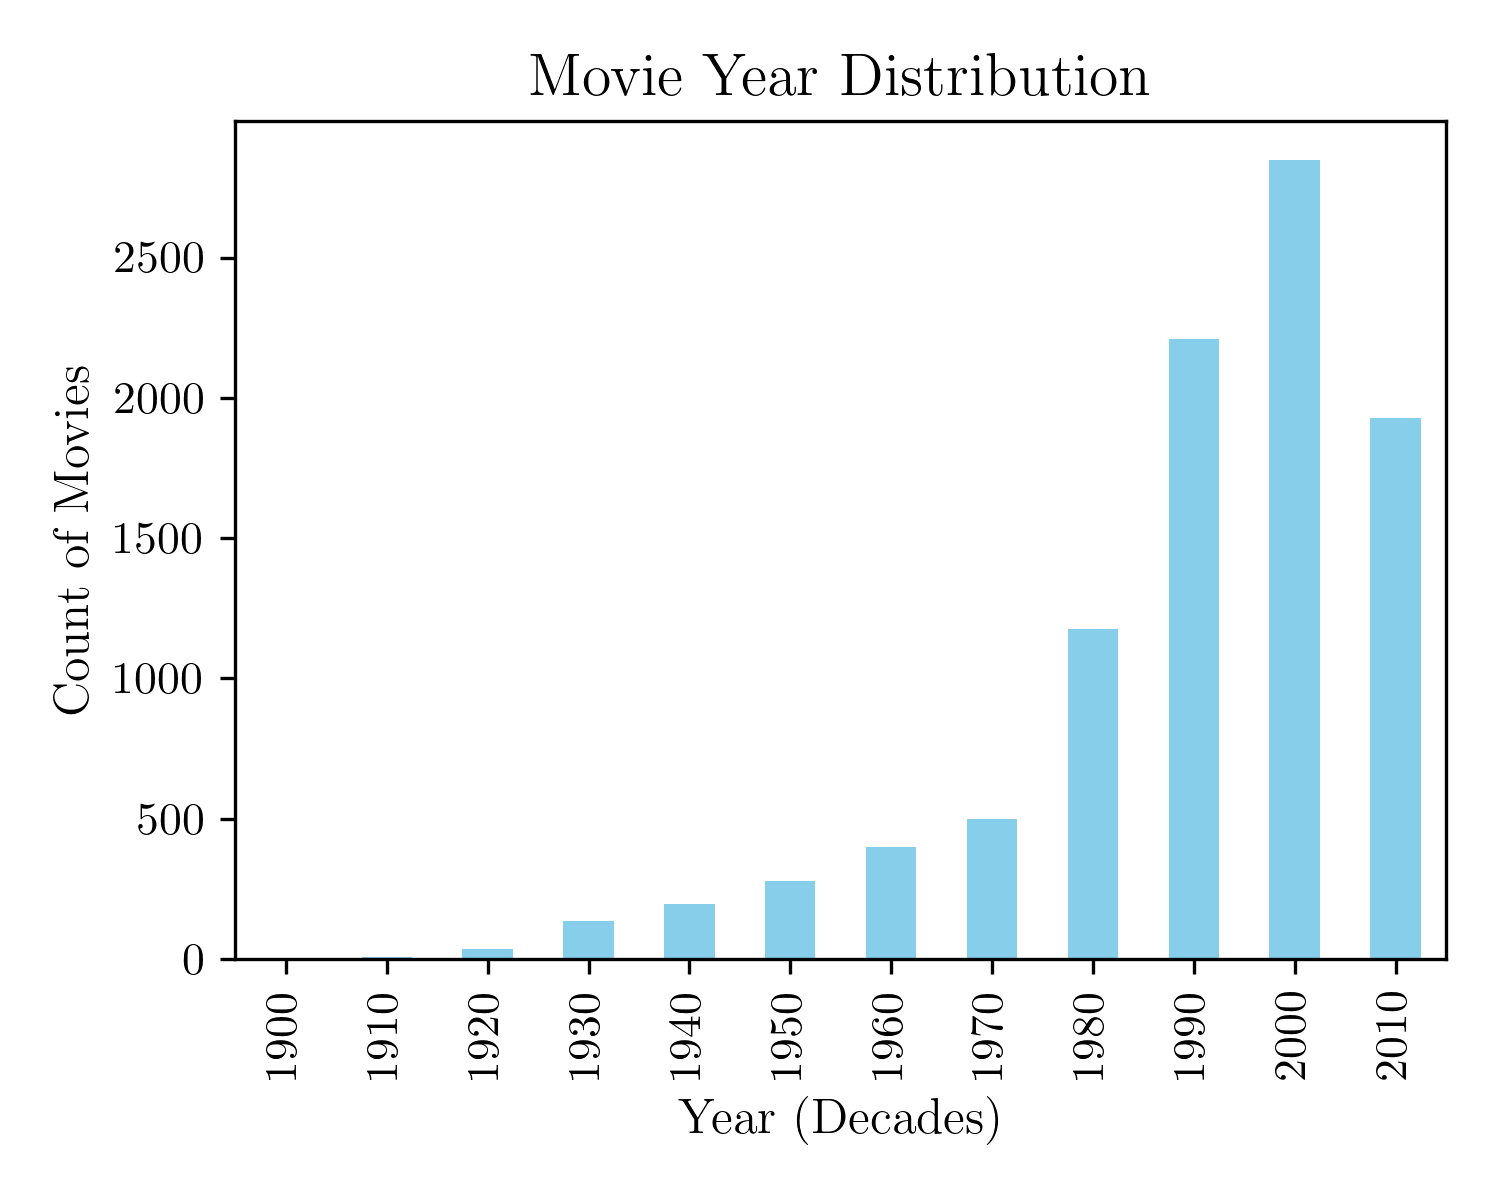
\includegraphics[width=1\linewidth]{assets/year_distribution.png}
    \caption{Movies distribution per year.}
    \label{fig:year_distribution}
\end{figure}

As expected, both distributions from Fig. \ref{fig:distribution_moviesratings} and \ref{fig:distribution_userratings} are positively skewed, since in general there are more people rating a small amount of movies, and the number of movies with higher counts of ratings tends to decrease rapidly (as there are very few, very popular movies).

This type of distribution is commonly found across recommender systems, and represents well the challenges posed to these algorithms: sparsity, whereas most of the matrix is empty (98.3 \% of missing values); bias, popular movies tend to dominate the analysis; and the long tail represents the challenge to make recommendations based on the large number of movies (or users) with very few ratings (or that rated few movies).

\begin{figure}[H]
    \centering
    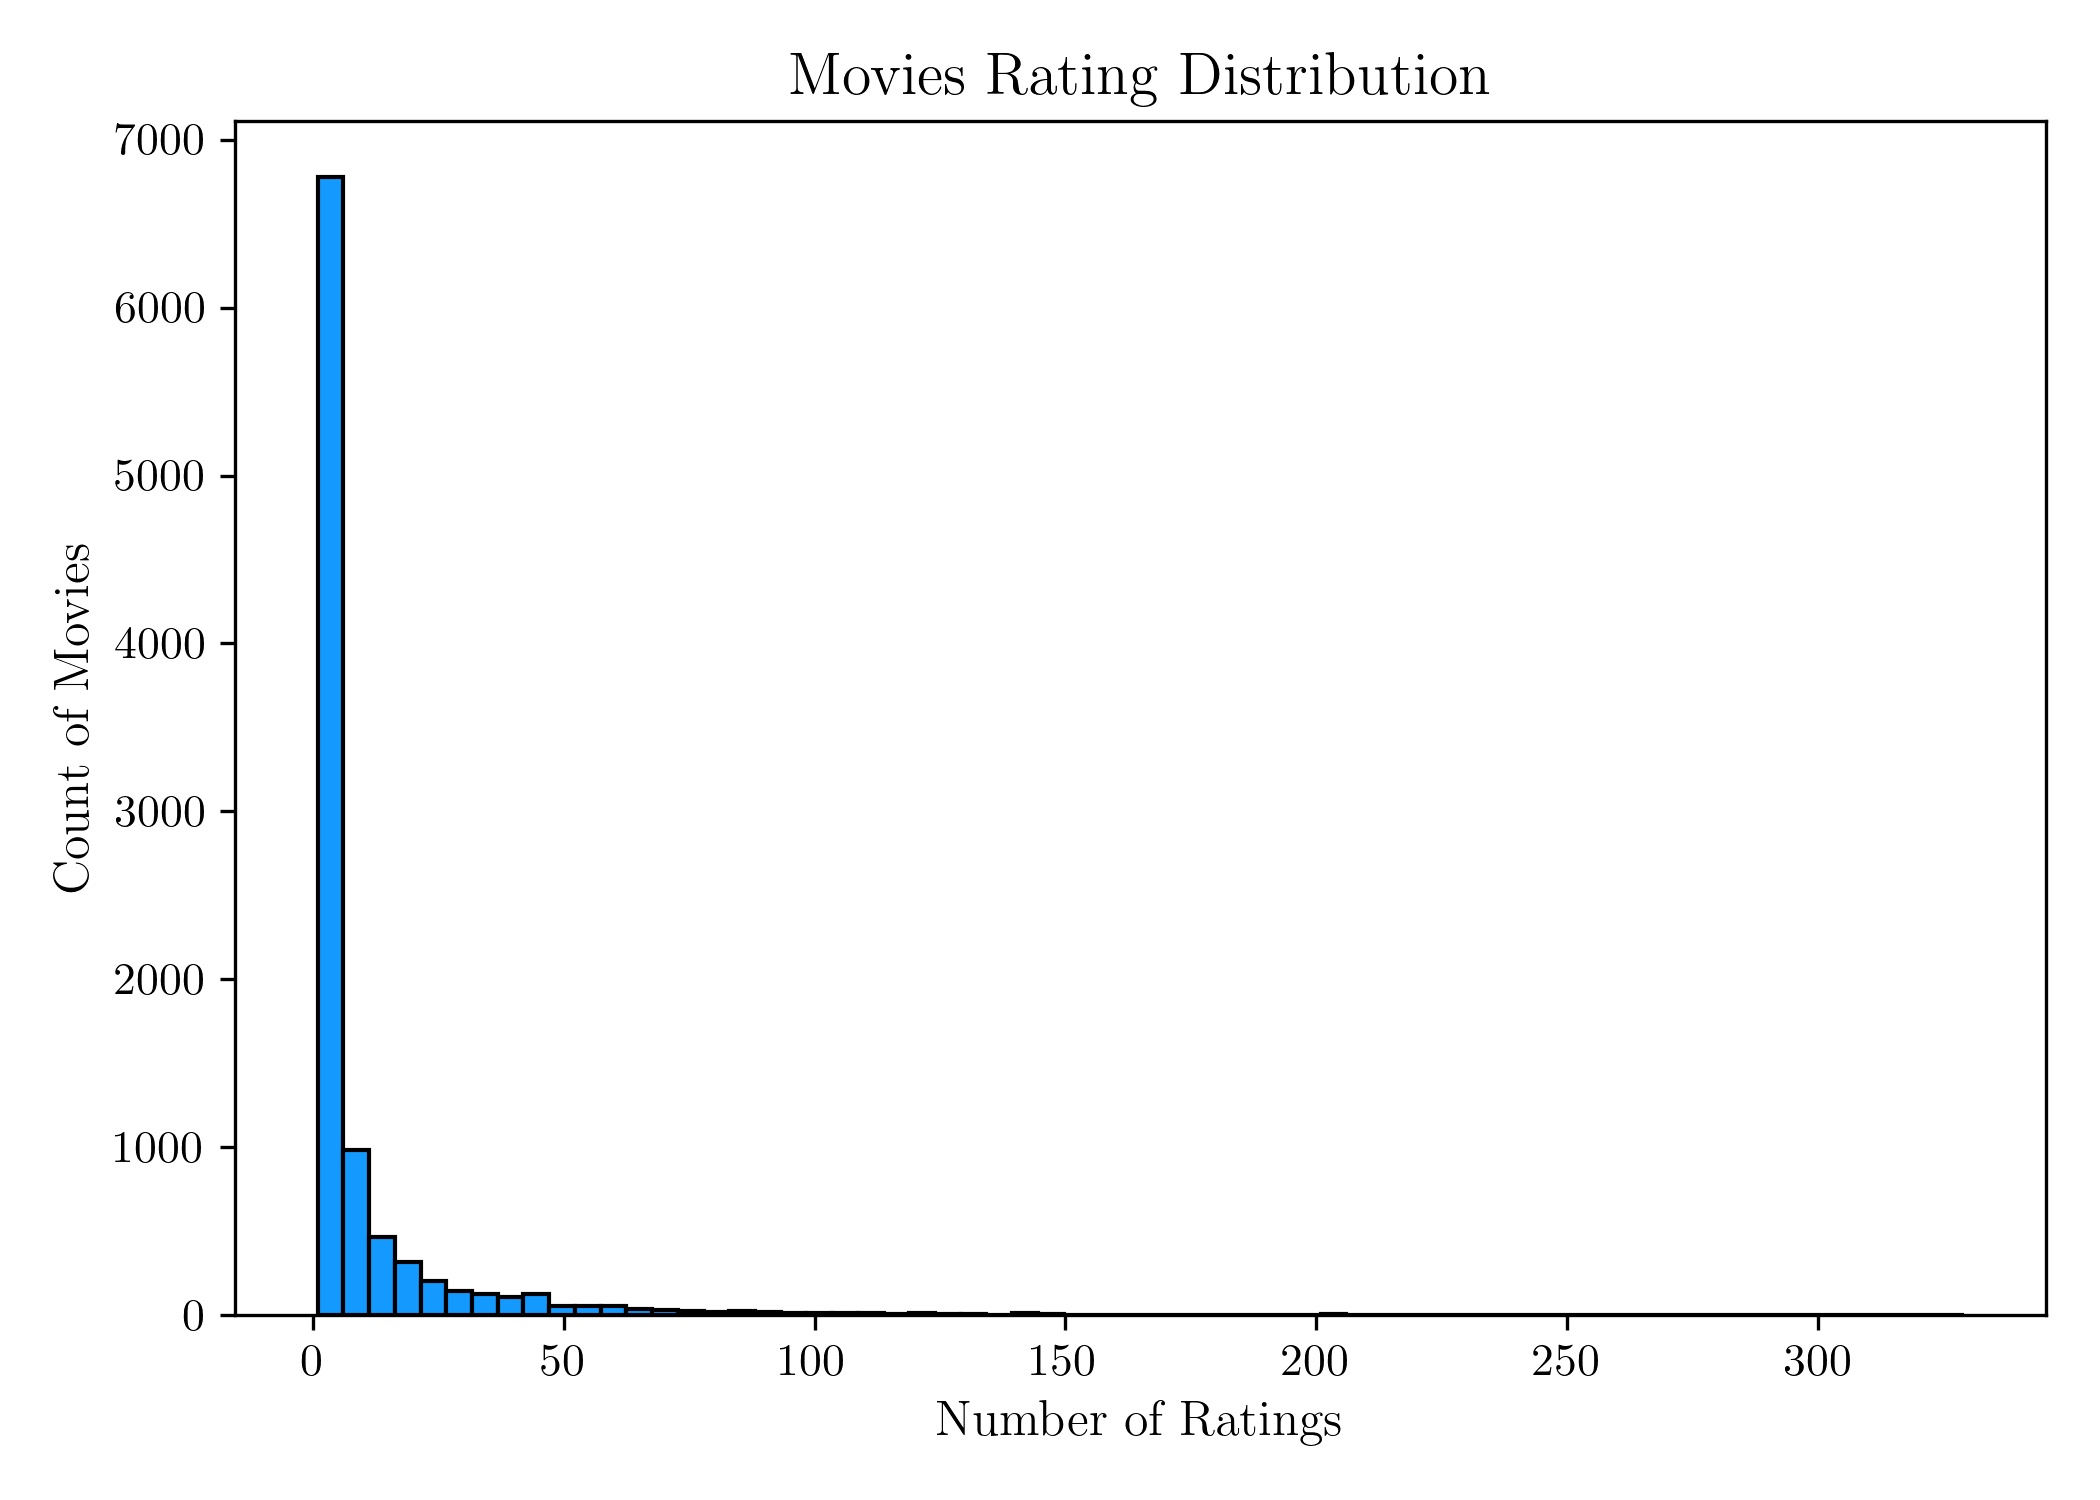
\includegraphics[width=1\linewidth]{assets/distribution_moviesratings.png}
    \caption{Distribution of movies based on the number of ratings, starting from 1 rating in the first bin.} 
    \label{fig:distribution_moviesratings}
\end{figure}

To finalize, it is important to mention (again) that the minimum number of ratings per user is 20, and the maximum is 2698. The minimum rating per movie is 1, and the maximum is 329 ratings. The most rated movies (and not so coincidentally) the highest rated movies were:
\begin{itemize}
    \item Forrest Gump (1994) - 329 ratings
    \item Pulp Fiction (1994) - 317 ratings
    \item The Shawshank Redemption (1994) - 307 ratings
\end{itemize}

\begin{figure}[h]
    \centering
    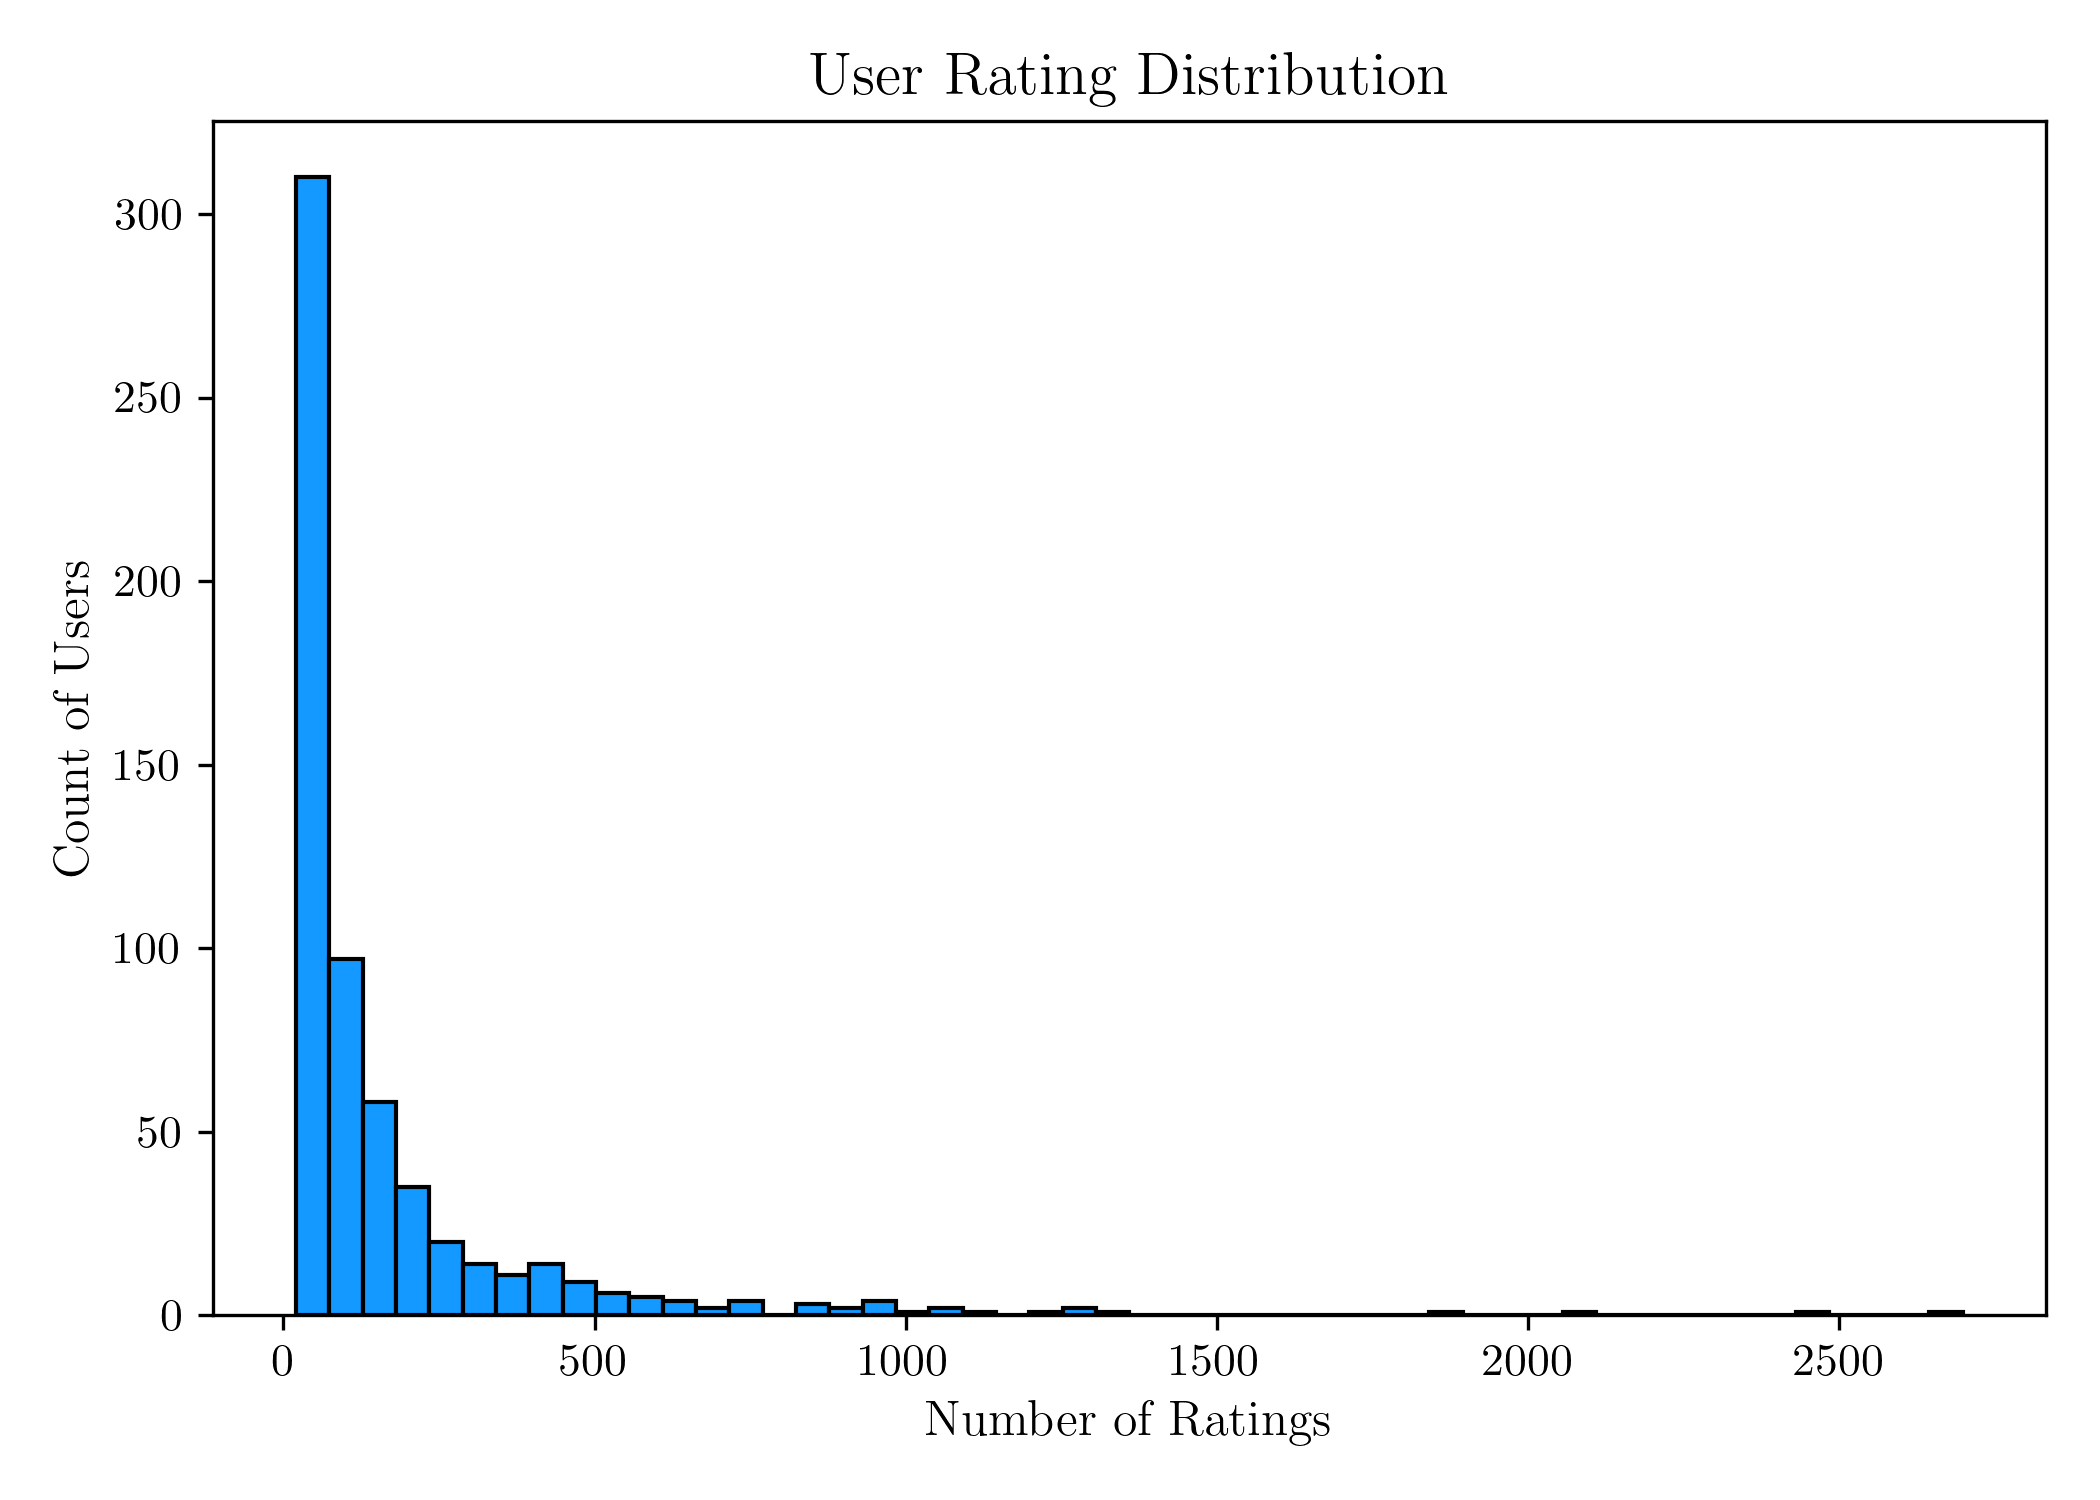
\includegraphics[width=1\linewidth]{assets/distribution_userratings.png}
    \caption{Distribution of users based on the number of ratings, starting from 20 ratings in the first bin.}
    \label{fig:distribution_userratings}
\end{figure}

\section{Classification Models}

The three models here presented are first and foremost linear regression problems, where by fitting a model with the known data to the users and the movies, it will be possible to estimate the ratings of movies that have not been reviewed. In this sense, besides the model itself, it is necessary to fit two hyperparameters, the learning rate $\alpha$, and the cost parameter $\lambda$. For both CF-LR and CB-LR 20 features were used for users, and for movies (40 features in total). The number of features was defined empirically, based on the number of genres in the dataset (20 genres).

The first model developed aims to fit both movies (\textit{x} parameter) and users ($\theta$ parameter) simultaneously, as depicted in the equation below, by optimization of the cost function with regularization.

\begin{multline}
\min_{\substack{x^{(1)}, \dots, x^{(n_m)} \\ \theta^{(1)}, \dots, \theta^{(n_u)}}} 
\frac{1}{2} \sum_{(i, j) : r(i, j) = 1} \left( (\theta^{(j)})^T x^{(i)} - y^{(i,j)} \right)^2 \\
+ \frac{\lambda}{2} \sum_{i=1}^{n_m} \sum_{k=1}^{n} \left( x_k^{(i)} \right)^2 + \frac{\lambda}{2} \sum_{j=1}^{n_u} \sum_{k=1}^{n} \left( \theta_k^{(j)} \right)^2
\end{multline}



The second model fits only the users parameter (20 features in total), given that it accounts for the movies parameters by using the movie genres.
\begin{align}
\min_{\theta^{(1)}, \dots, \theta^{(n_u)}} 
&\frac{1}{2} \sum_{j=1}^{n_u} \sum_{i : r(i, j) = 1} \left( (\theta^{(j)})^T x^{(i)} - y^{(i,j)} \right)^2 \notag \\
&+ \frac{\lambda}{2} \sum_{j=1}^{n_u} \sum_{k=1}^{n} \left( \theta_k^{(j)} \right)^2
\end{align}

The third and final model is the famous FunkSVD. As mentioned in the state of the art, despite the many regularization parameters, we've limited the analysis to the number of latent features, overall learning rate (which could be fit for the many features possible), and the regularization parameters.

\subsection{CF-LR Model}

Different ranges of $\alpha$ (between 0.0001 and 0.002) and $\lambda$ (between 0 and 100) were given to the model to be fit by using 8 cross-validation in the training dataset. This allowed to progressively lower RMSE, throughout 500 iterations.

The best hyperparameters for this model were $\lambda = 6$ and $\alpha = 0.0005$, with an average RMSE from 8-fold CV of 1.25622.

\begin{figure}[H]
    \centering
    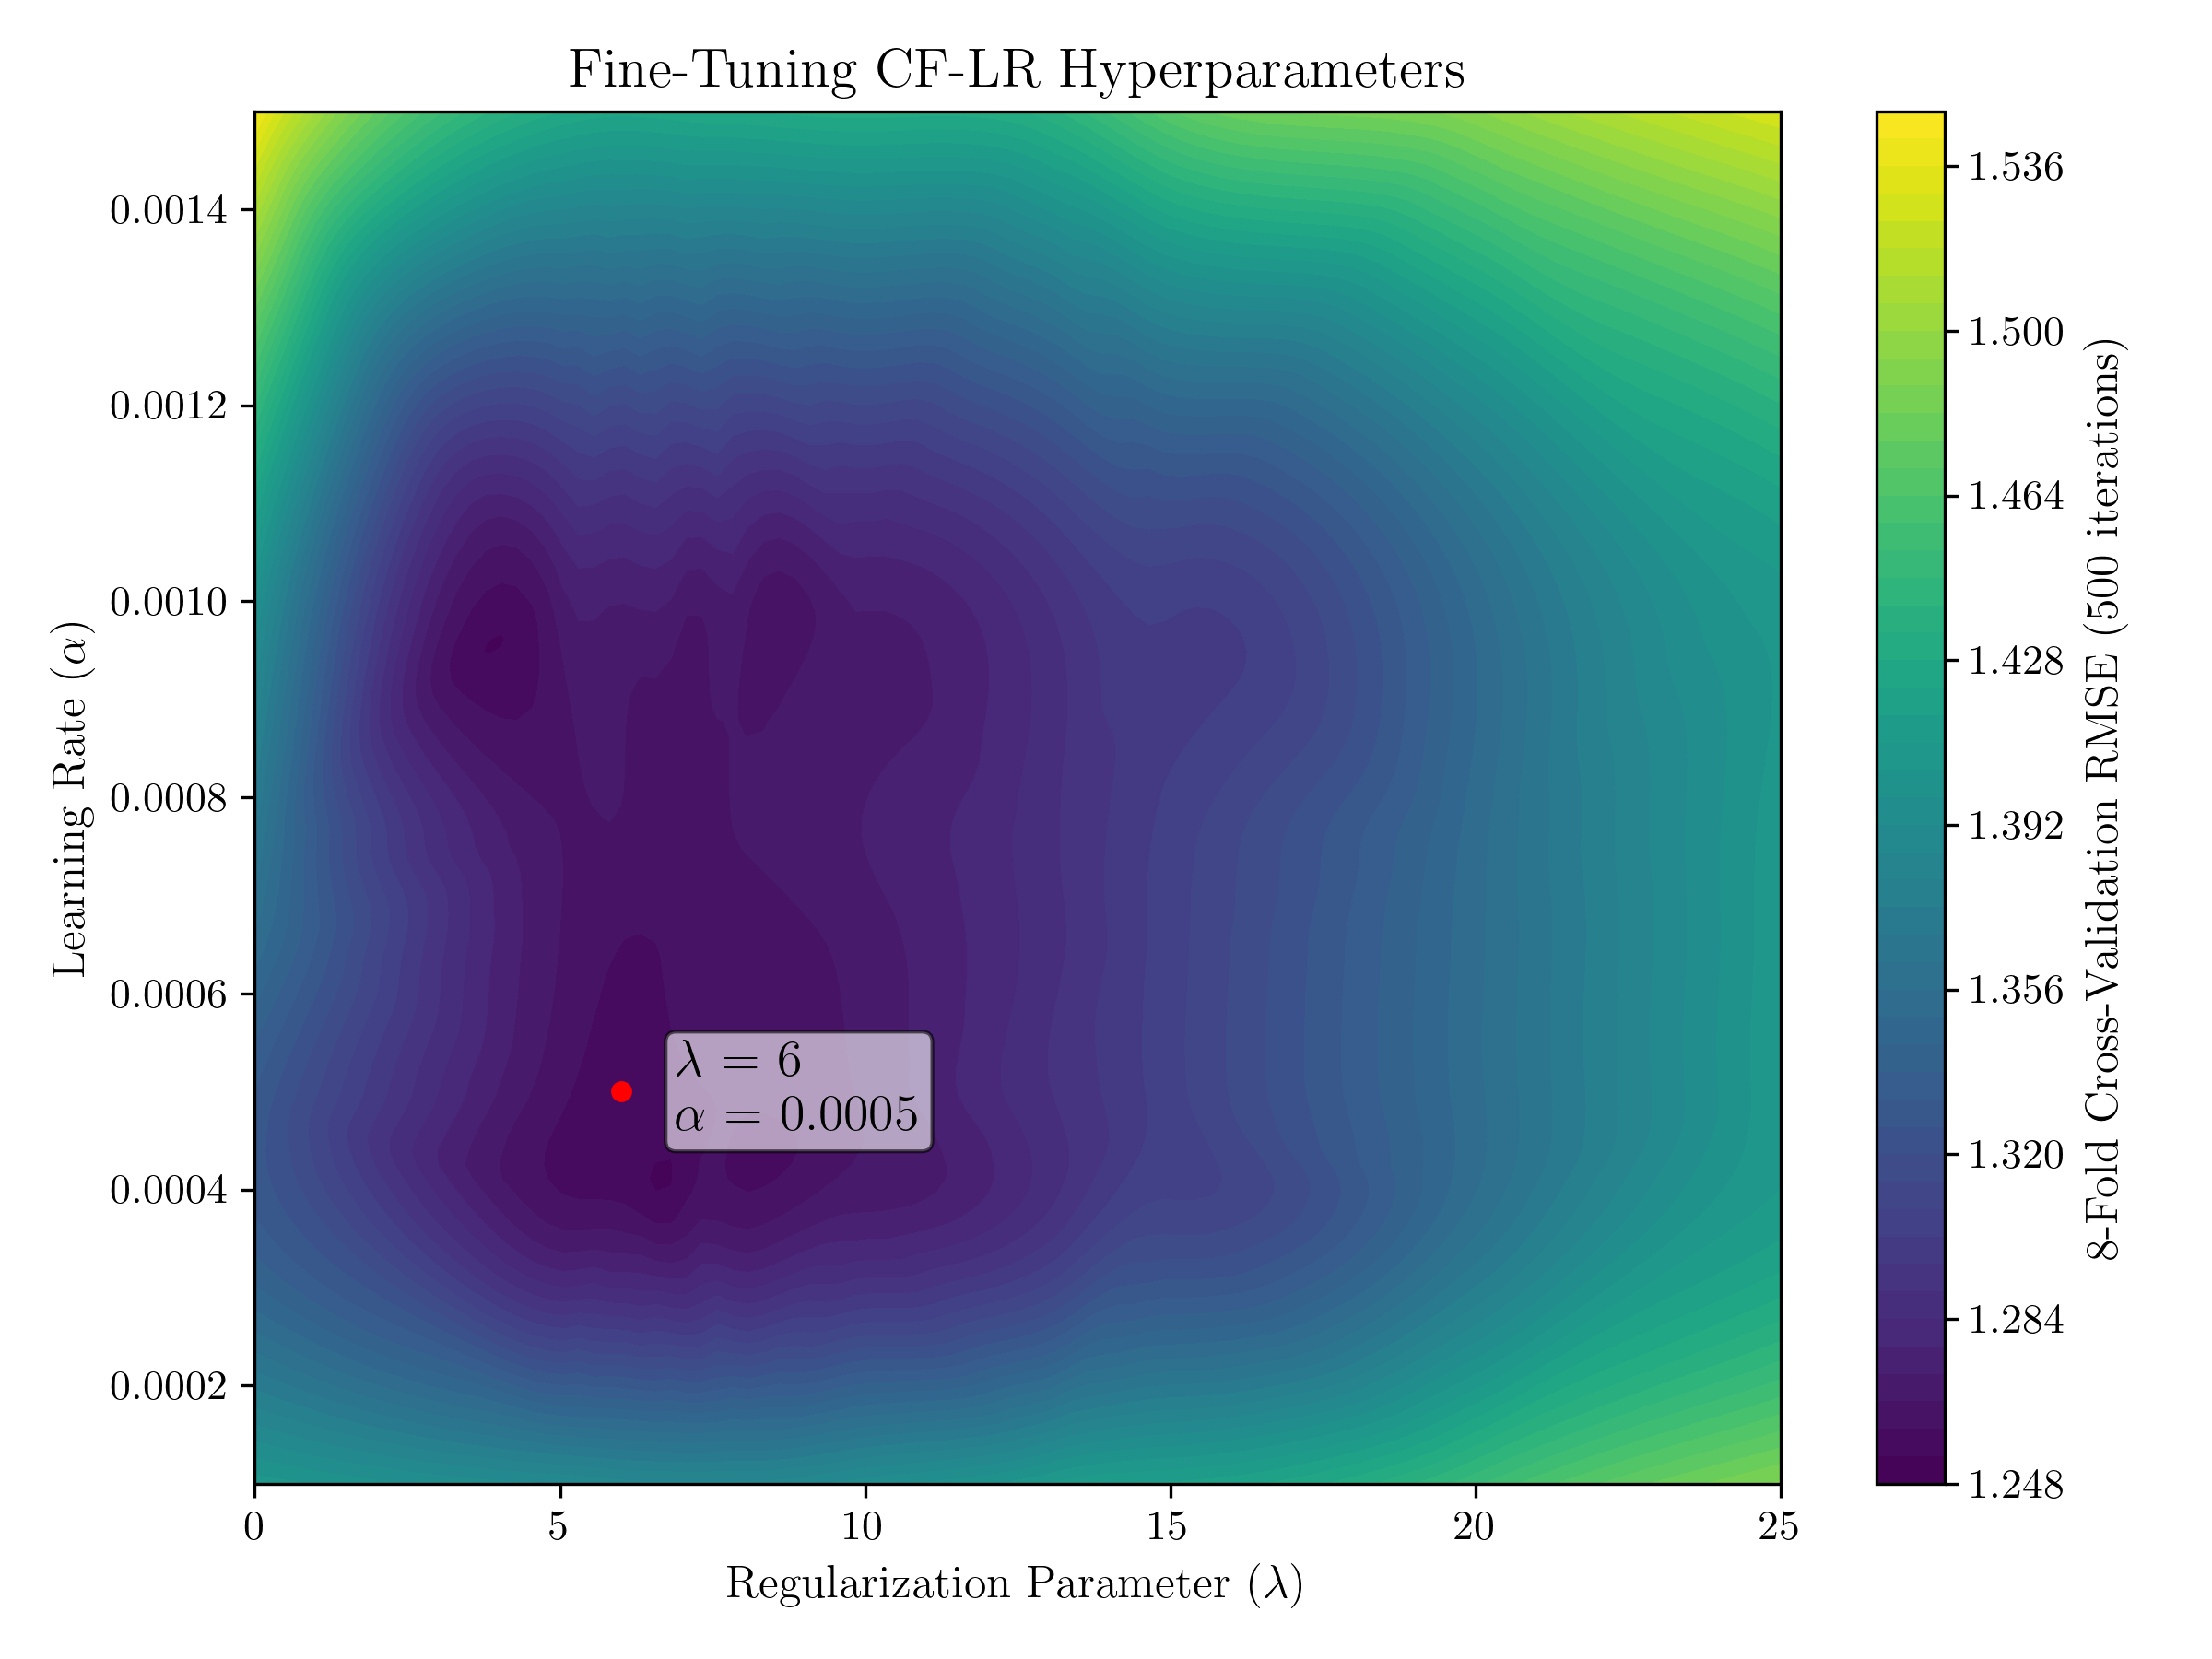
\includegraphics[width=1\linewidth]{assets/model01_hyperparametres.png}
    \caption{Learning rate ($\alpha$) and regularization parameter ($\lambda$) fine-tuning for the CF-LR model.}
    \label{fig:model01_hyperparametres}
\end{figure}

Once the optimal hyperparameters were defined, the learning curve was estimated from the 8-fold CV on the training dataset, to assess the validity of the model and that it is not overfit. In Fig. \ref{fig:model01_learning_curve} the progression of the training score and the CV score tends to improve across the train set size, not overlapping or changing the trend significantly. It is important to bear in mind that there is a risk of slight overfitting, considering that there are 40 features to be fit.

\begin{figure}[H]
    \centering
    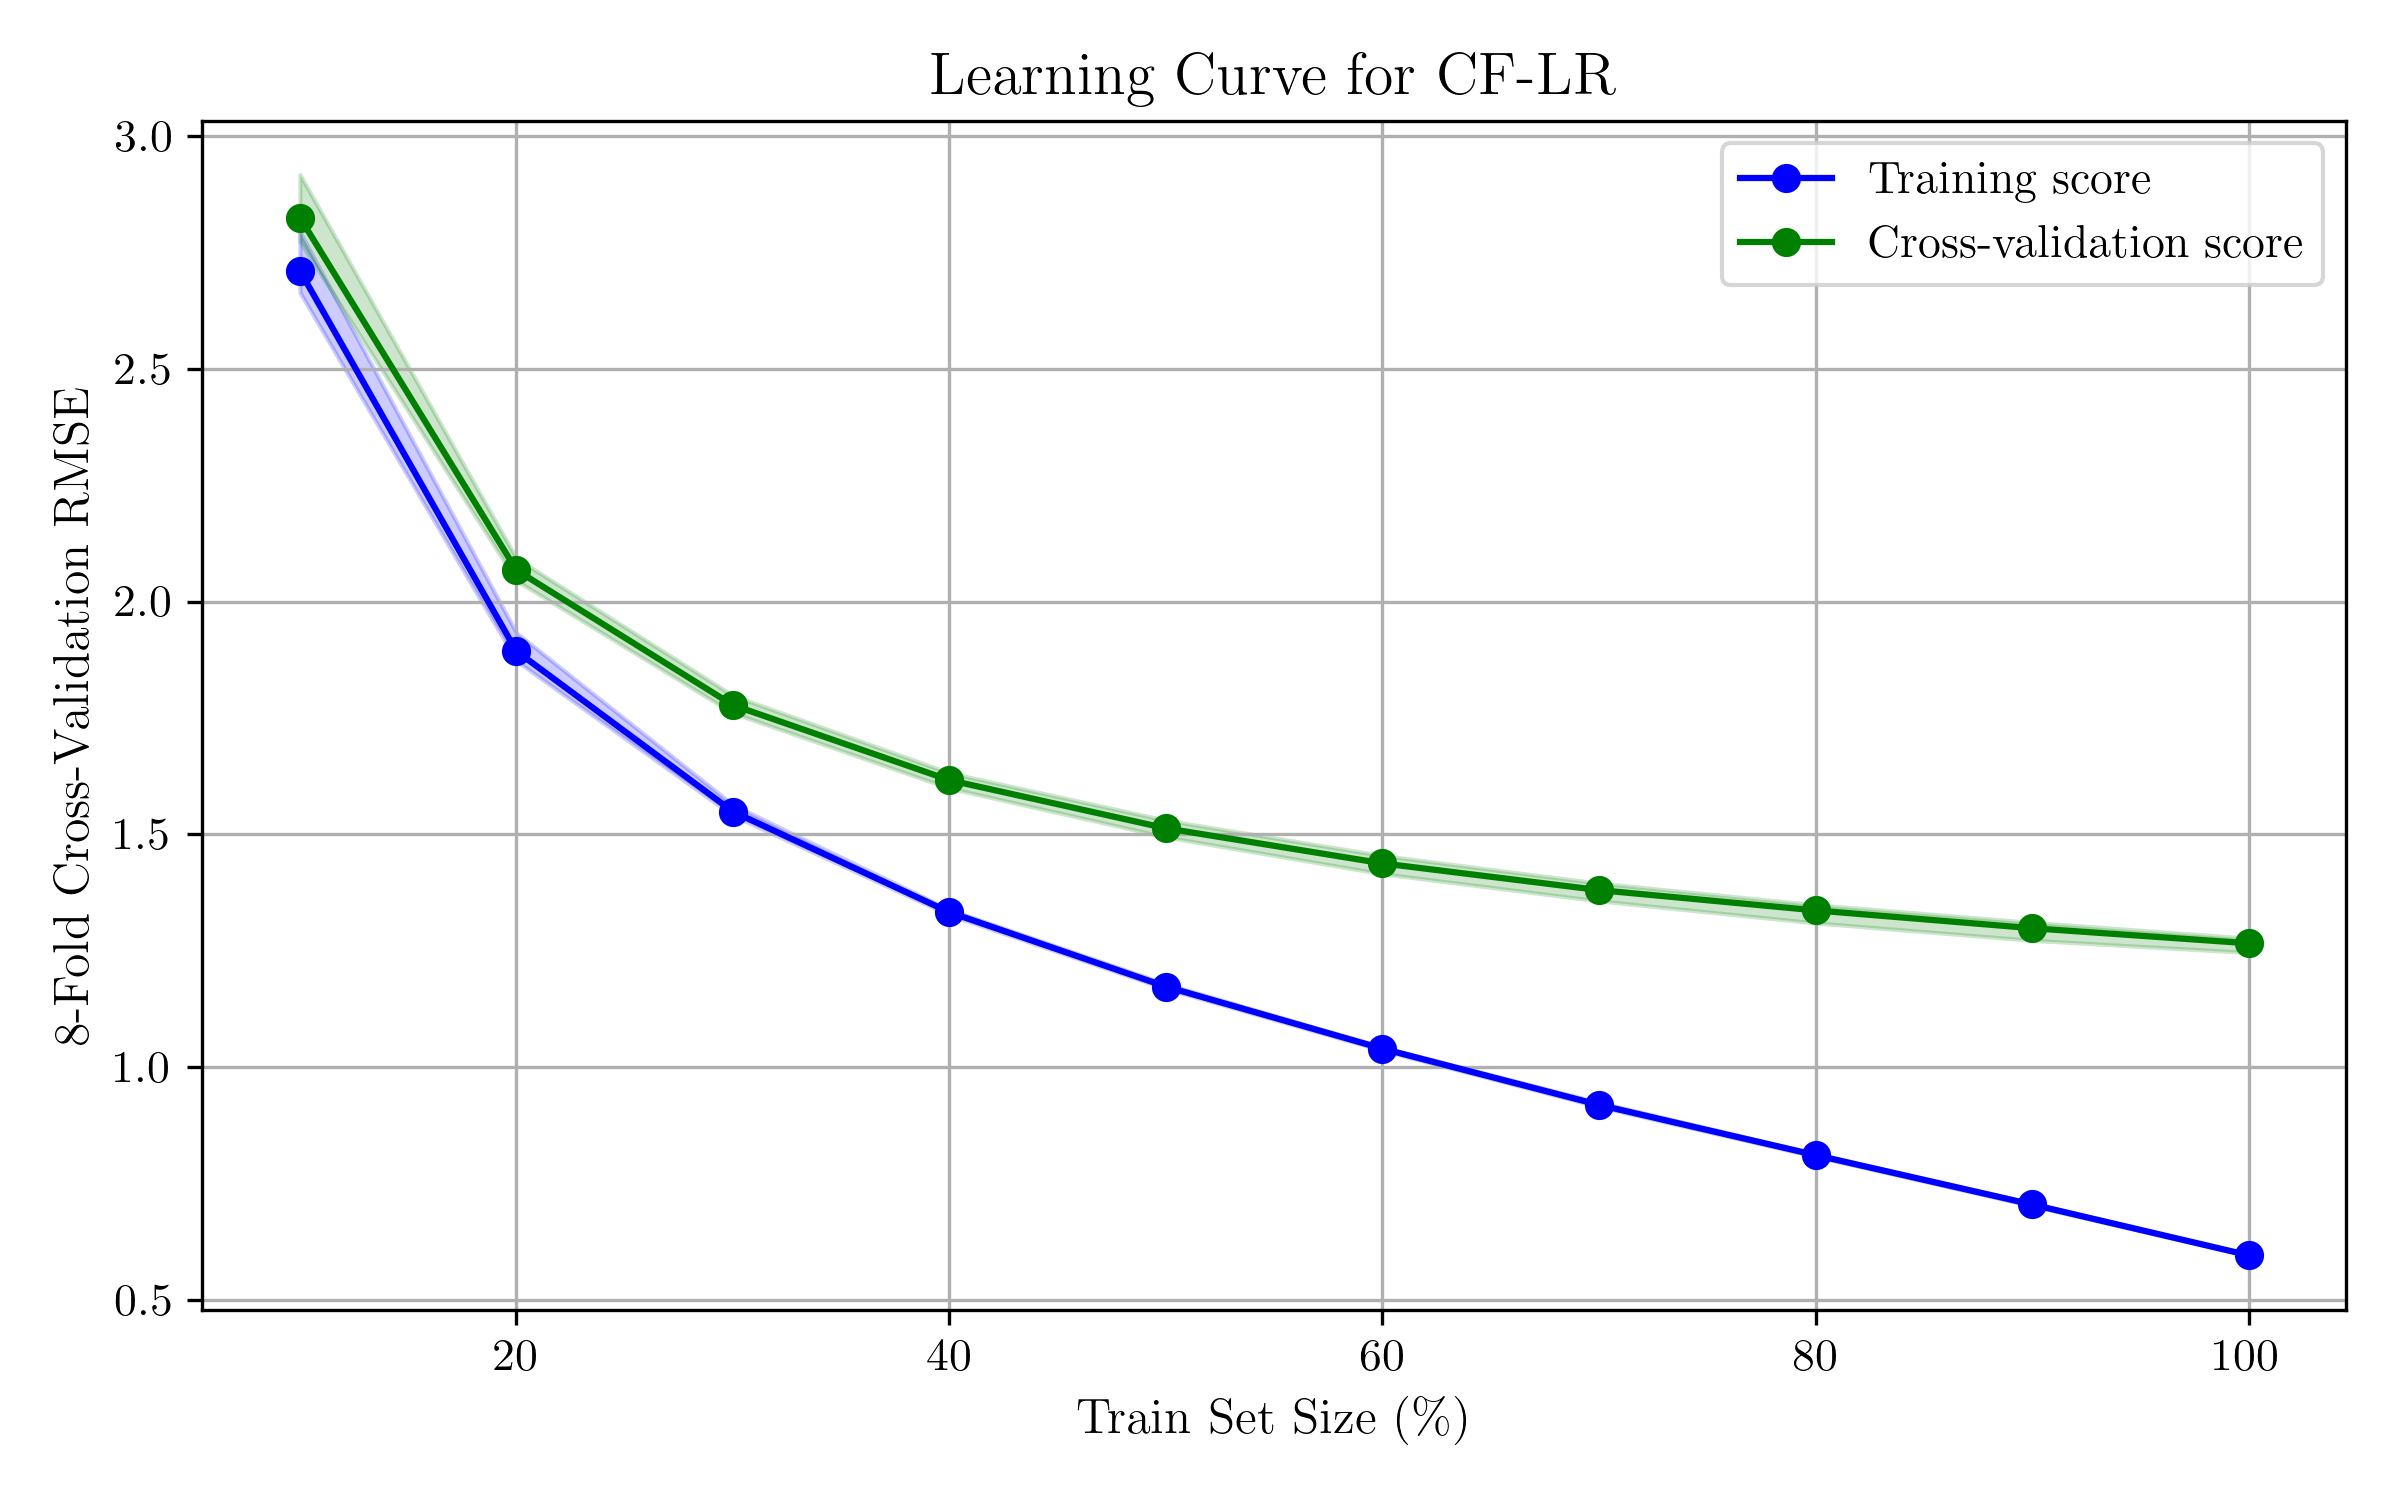
\includegraphics[width=1\linewidth]{assets/model01_learning_curve.png}
    \caption{CF-LR learning curve: 8-fold CV RMSE progression throughout the training dataset.}
    \label{fig:model01_learning_curve}
\end{figure}

Using the defined hyperparameters, the cost function was estimated, where we see it sharply decreasing as the iterations run, finally converging at the limit.

\begin{figure}[H]
    \centering
    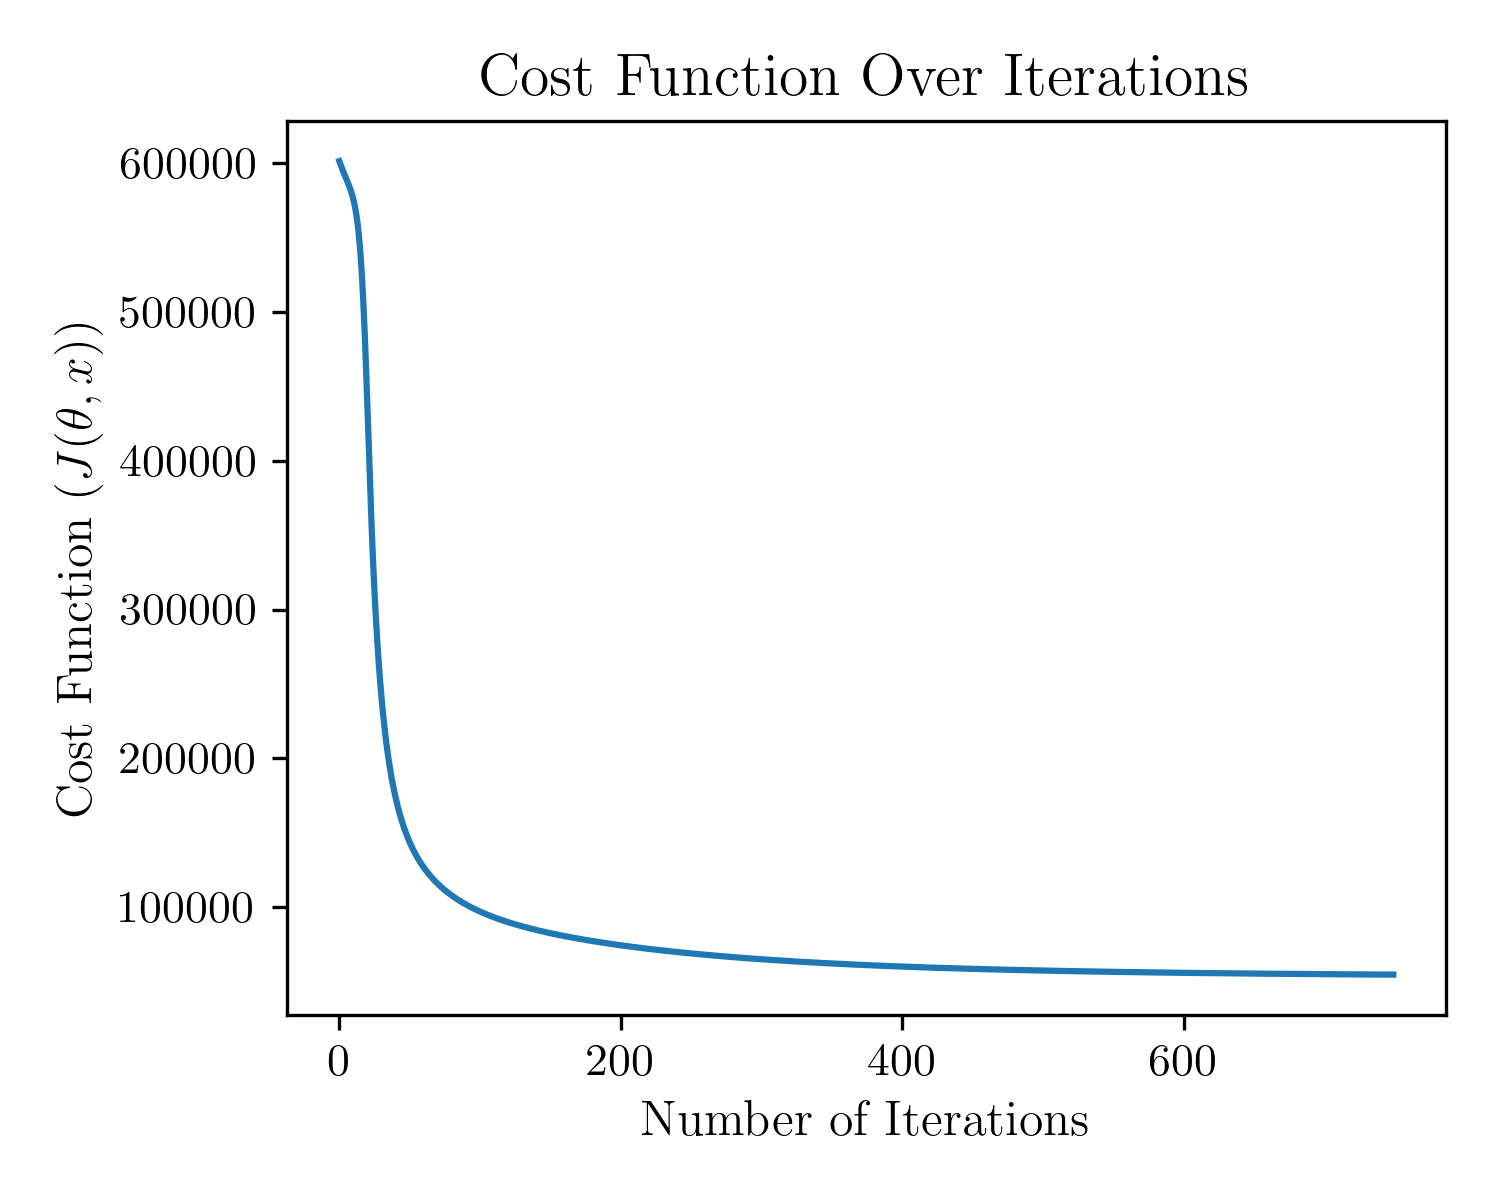
\includegraphics[width=1\linewidth]{assets/model01_cost_function.png}
    \caption{Evolution of the CF-LR model's cost function over iterations.}
    \label{fig:model01_cost_function}
\end{figure}

With the model defined, the train and test sets were compared for the errors (RMSE and MAE), as depicted in Table \ref{tab:model01_results}, showing an increase of errors in the test set in regards to the training set. The fact that errors increased significantly from the training to the testing set supports the likelihood of overfitting the data.

\begin{table}[H]
\centering
\caption{Error metrics for the train and test set (CF-LR), along with the number of samples for each.}
\label{tab:model01_results}
\begin{tabular}{lccc}
\toprule
\textbf{Dataset} & \textbf{RMSE} & \textbf{MAE} & \textbf{Support} \\
\midrule
Train Set & 0.58842 & 0.44604 & 80668 \\
Test Set & 1.24037 & 0.90651 & 20168 \\
\bottomrule
\end{tabular}
\end{table}

\subsection{CB-LR Model}

The CB-LR model is less demanding as it is only estimating the features related to the users, considering that the movie features are estimated from the genres given per movie in the dataset. Each movie is weighted in terms of how much it is represented by a given genre (e.g., Pearl Harbor being for example 33/33/33: war, drama and romance), which is represented by vector \textit{x}. The movie features don't need to be optimized, and as the name states, the model is a linear regression \textit{content based}, leaving the vector \textit{$\theta$}, user features, to be optimized. 

As seen in Fig. \ref{fig:model02_hyperparemeterstunning}, $\alpha$ was optimized between 0.00005 and 0.007, whereas $\lambda$ was varied between 0 and 10. The optimized hyperparameters (as a result of 8-fold CV) are pinpointed in the graph, corresponding to (0.05, 0.005) with 8-fold CV RMSE of 0.98617.

\begin{figure}[H]
    \centering
    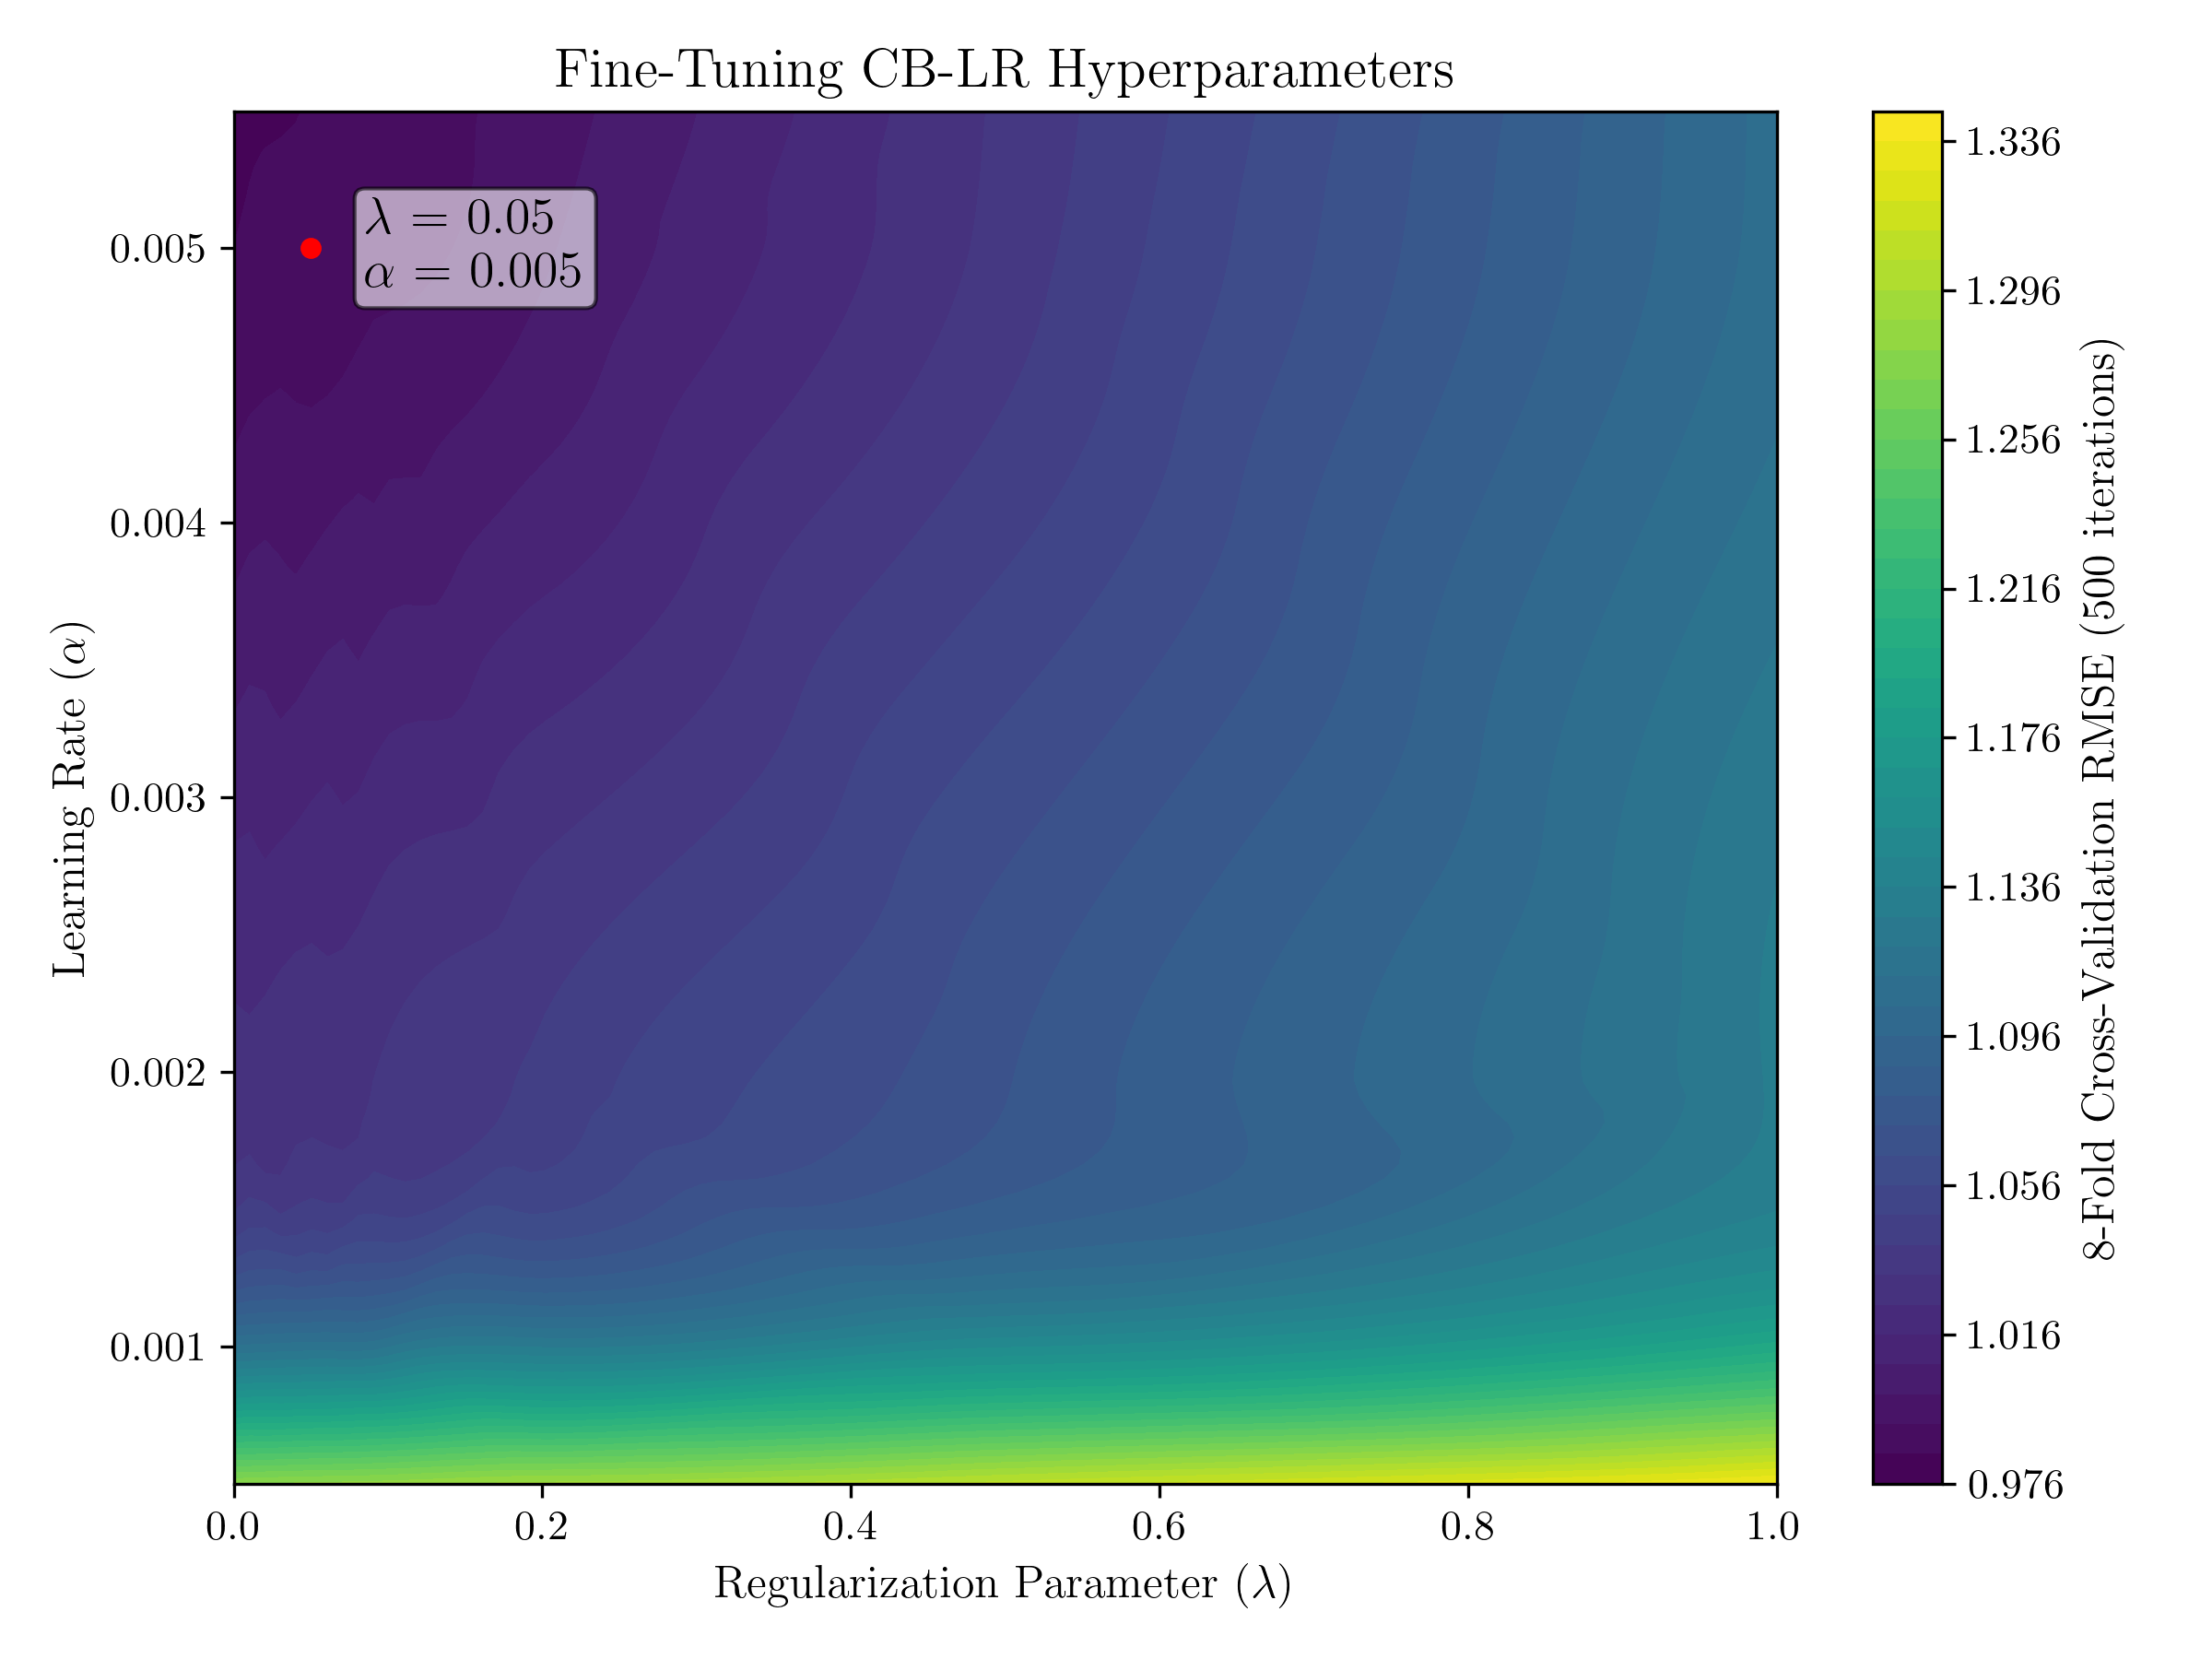
\includegraphics[width=1\linewidth]{assets/model02_hyperparemeterstunning.png}
    \caption{Learning rate ($\alpha$) and regularization parameter ($\lambda$) fine-tuning for CB-LR model.}
    \label{fig:model02_hyperparemeterstunning}
\end{figure}


As in CF-LR the learning curve was estimated to ensure no overfitting occurred. In this case the trends vary in an identical fashion for the whole training set, which is a good indicator of an adequate fit. 

\begin{figure}[H]
    \centering
    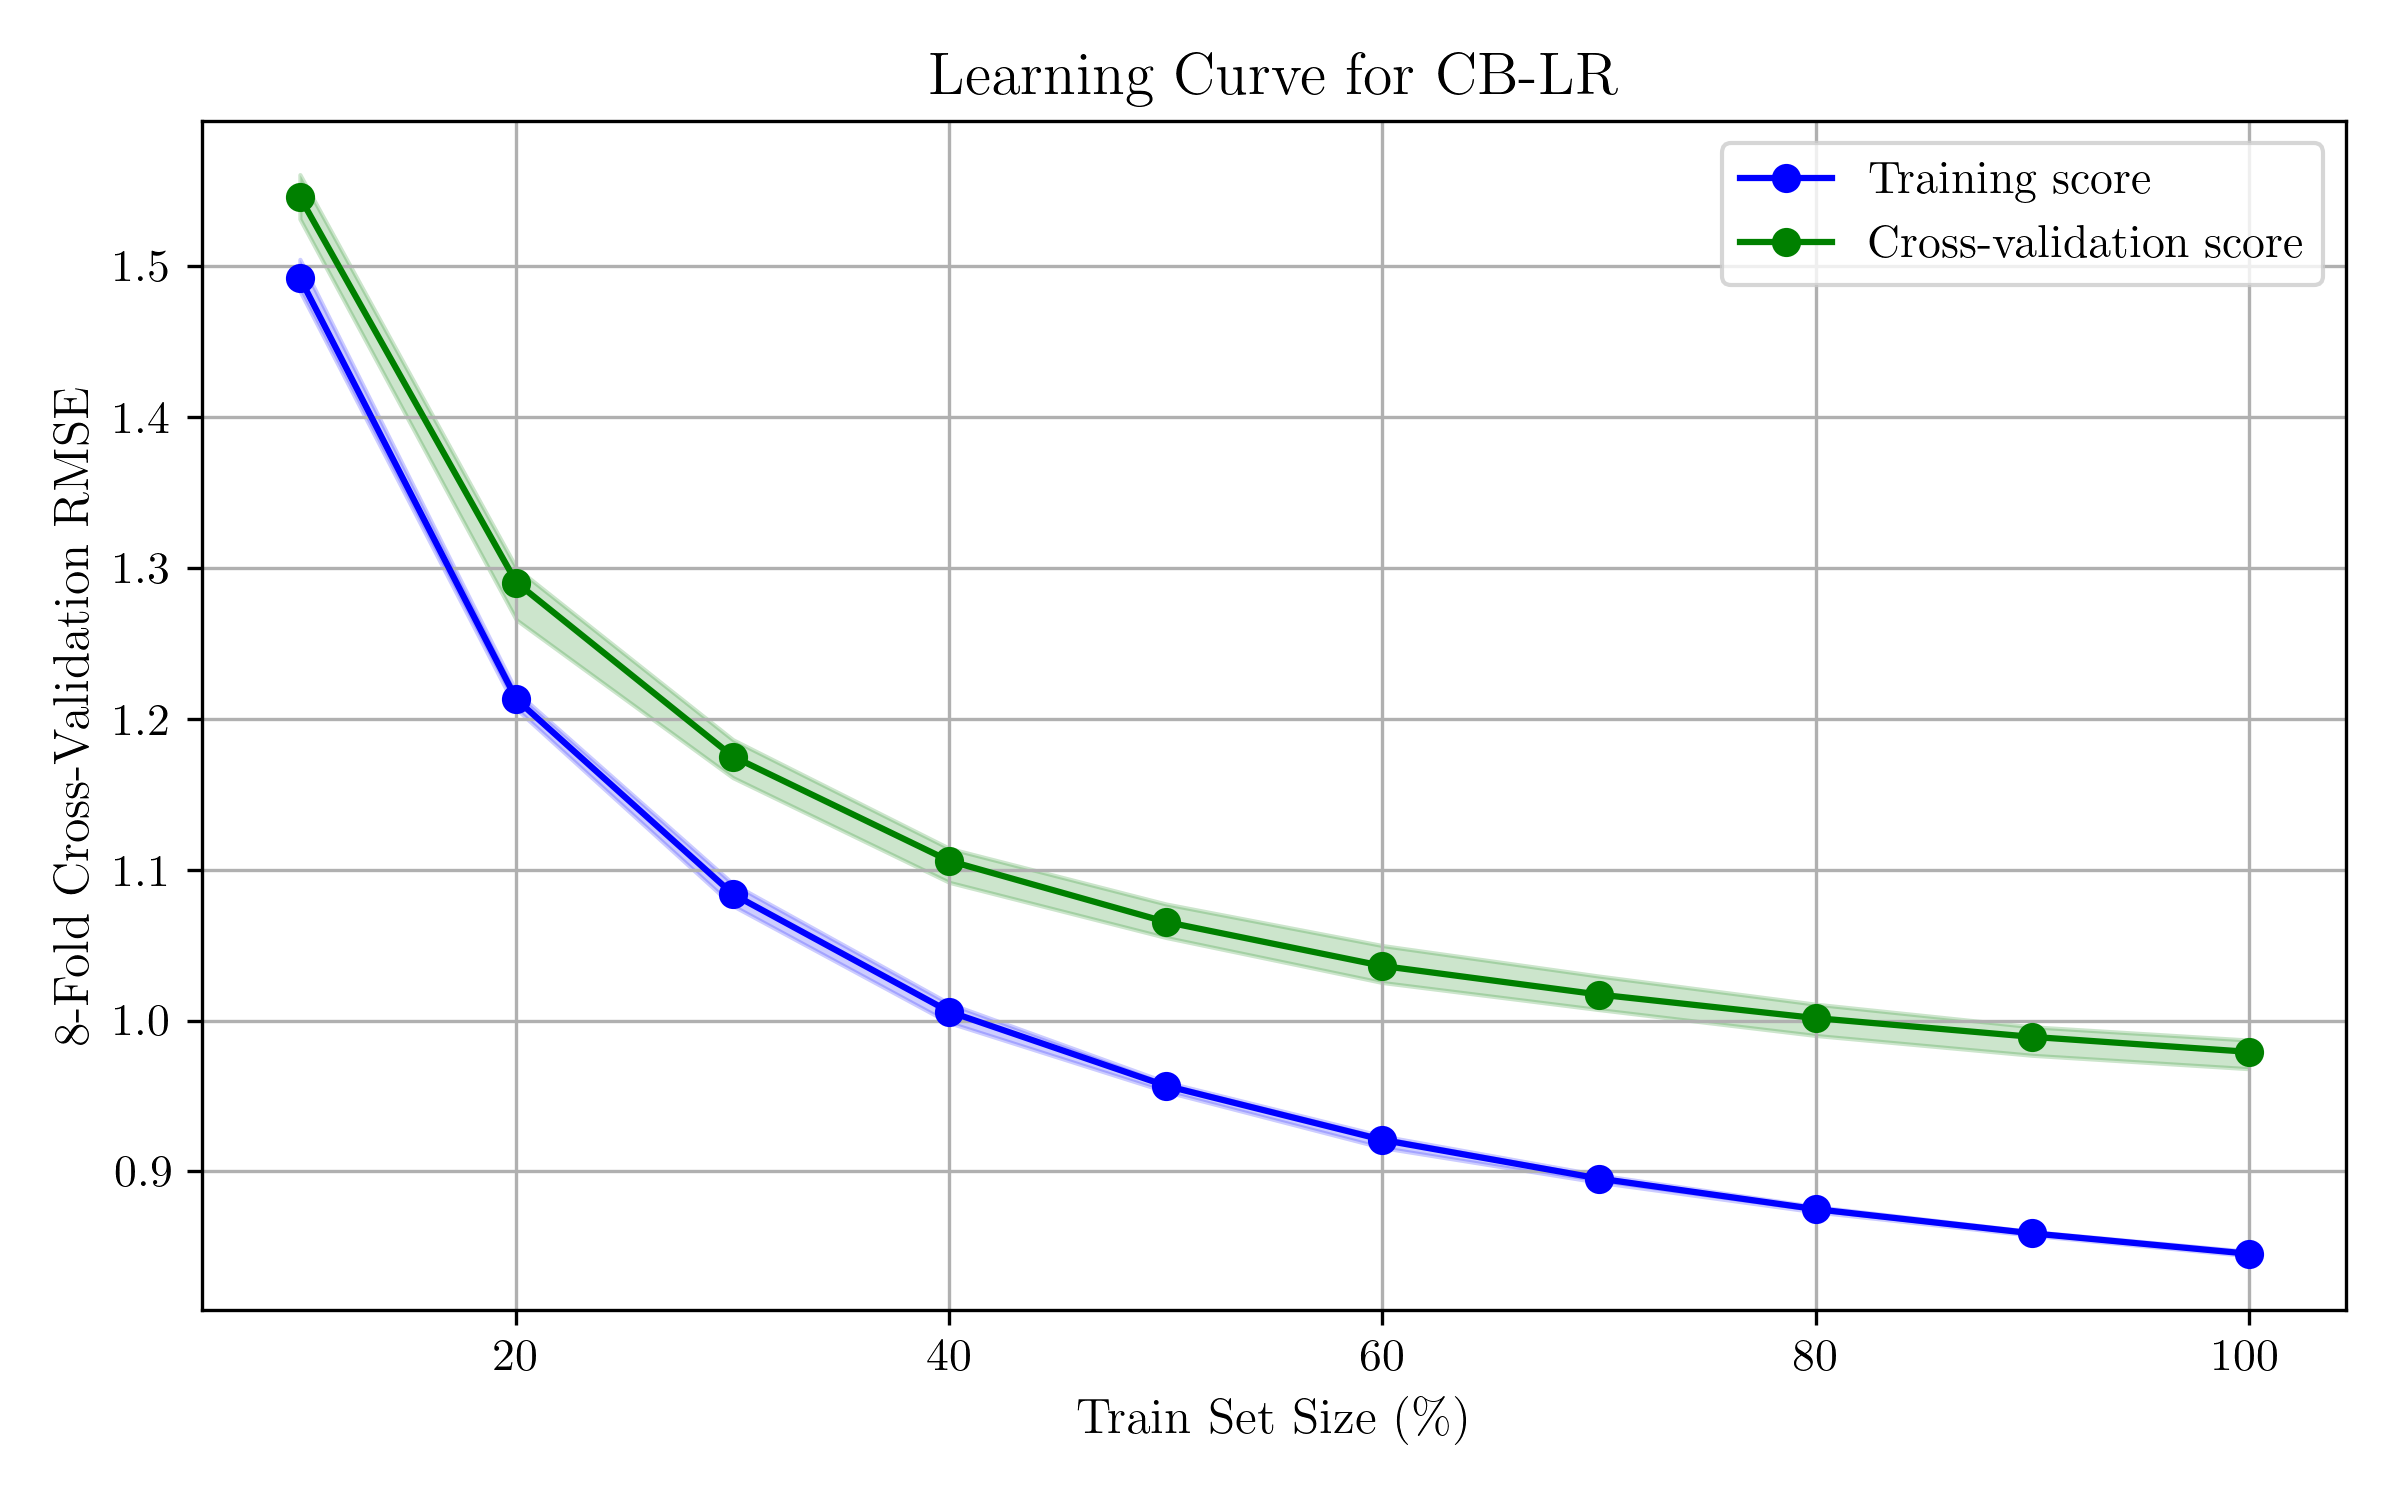
\includegraphics[width=1\linewidth]{assets/model02_learning_curve.png}
    \caption{CB-LR learning curve: 8-fold CV RMSE progression throughout the training dataset.}
    \label{fig:model02_learning_curve}
\end{figure}

In Fig. \ref{fig:model02_cost_function} the cost function is minimized as in CF-LR, indicating proper convergence of the model.

\begin{figure}[H]
    \centering
    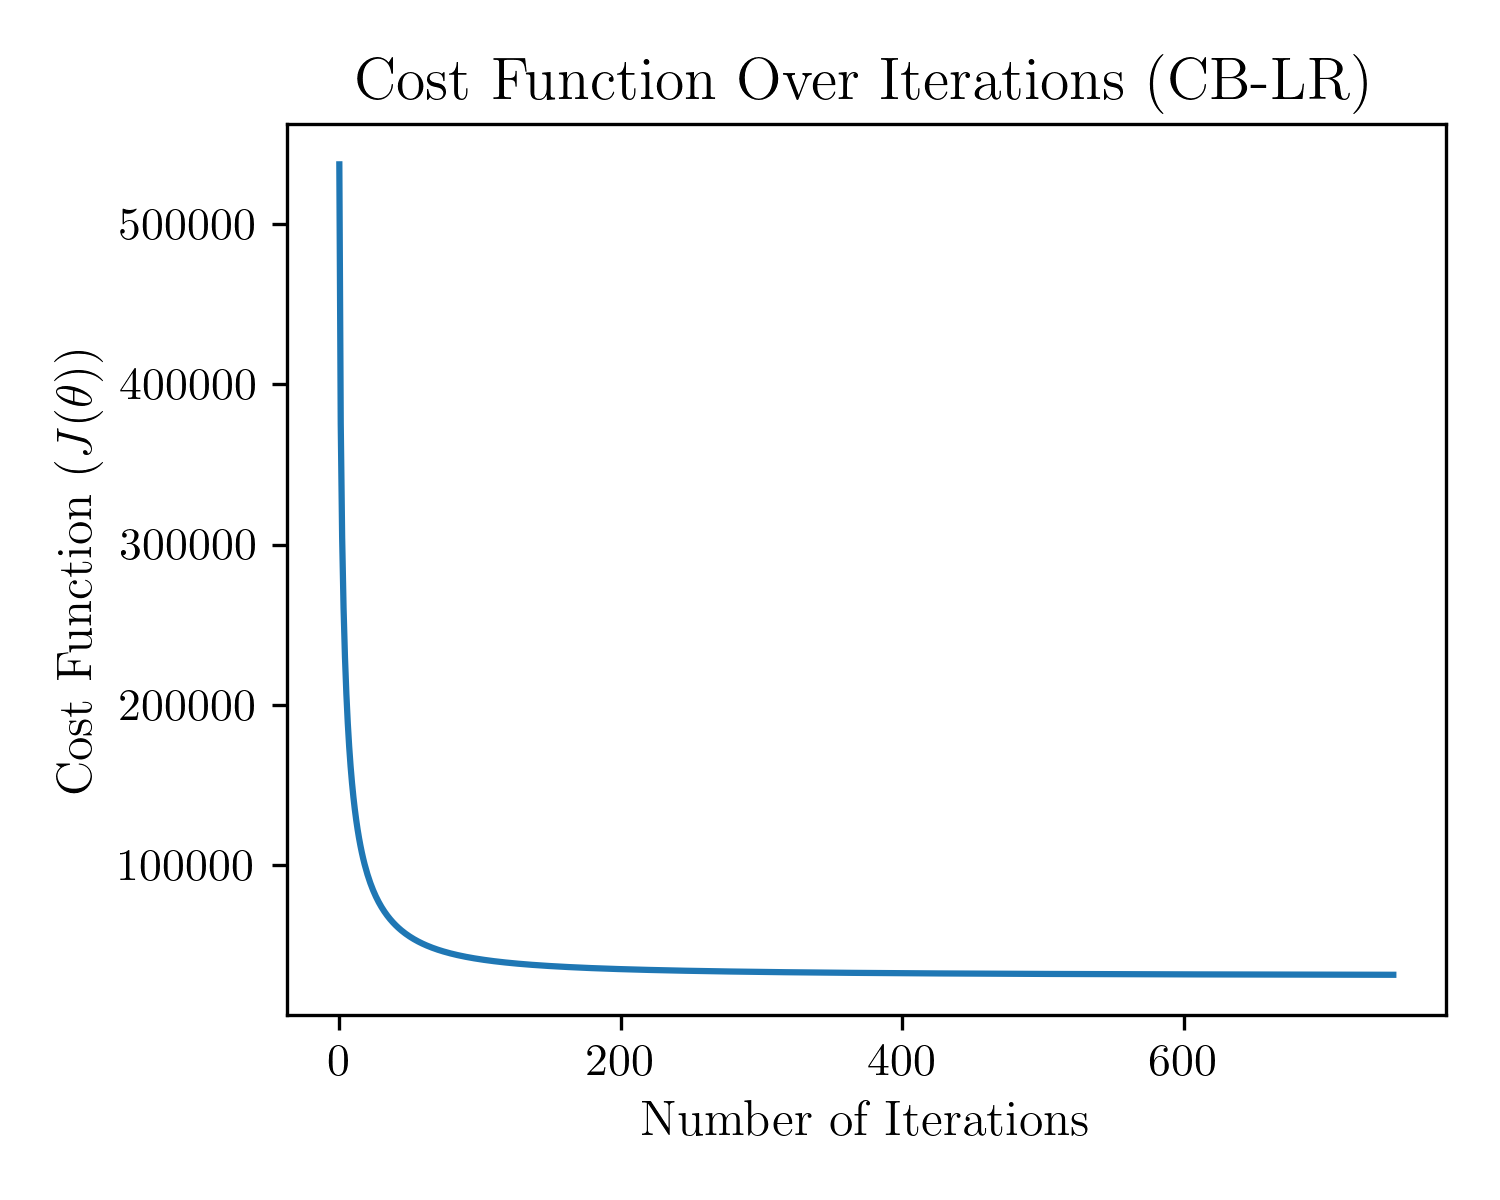
\includegraphics[width=1\linewidth]{assets/model02_cost_function.png}
    \caption{Evolution of the CB-LR model's cost function over iterations.}
    \label{fig:model02_cost_function}
\end{figure}

The error metrics in Table \ref{tab:model03_results} further contribute to the model's proper fit, that do not vary significantly from the train to the test set.

\begin{table}[H]
\centering
\caption{Error metrics for the train and test set (CB-LR), along with the number of samples for each.}
\label{tab:model03_results}
\begin{tabular}{lccc}
\toprule
\textbf{Dataset} & \textbf{RMSE} & \textbf{MAE} & \textbf{Support} \\
\midrule
Train Set & 0.84859 & 0.65997 & 80668 \\
Test Set & 0.97254 & 0.74605 & 20168 \\
\bottomrule
\end{tabular}
\end{table}

\subsection{CF-FunkSVD Model}

The CF-FunkSVD model was designed with a minimal set of optimized hyperparameters to reduce the risk of overfitting and to evaluate the impact of these parameters on the model's performance. The optimization process was conducted using a \textit{GridSearchCV} with an 8-fold cross-validation. In Table \ref{parametrosSVD} the range of values for each hyperparameter is given, where \textit{n\_factors} corresponds to the number of factors, \textit{lr\_all} is the overall learning rate, and \textit{reg\_all} the regularization parameter. The remaining parameters are kept as default, indicated in \textit{surprise} Python package \cite{surprise}. The best fit values were 50, 0.01, and 0.1, respectively.

\begin{table}[H]
\centering
\caption{CF-FunkSVD model hyperparameters search space.}
\label{parametrosSVD}
\begin{tabular}{ll}
\toprule
\textbf{Hyperparameter} & \textbf{Possible Values} \\
\midrule
$n\_factors$ & \{$5,15,30,40,50$\} \\ 
$lr\_all$ & \{$0.005, 0.01, 0.05, 0.1, 1$\} \\ 
$reg\_all$ & \{$0.02,0.1,1,5,10$\} \\ 
\bottomrule
\end{tabular}
\end{table}

The learning curve (Fig. \ref{fig:model03_learningcurve}) shows a different behavior considering what was observed in the other two models, where both training and testing are converging, with the former evidencing increasing RMSE, while the latter presenting a decreasing trend.

With this sort of approach, as the training set increases the model becomes more generalist, while compromising its accuracy, resulting in an increased error. The fact that the testing set shows decreasing RMSE is a sign that the model is able to be more generic.

\begin{figure}[H]
    \centering
    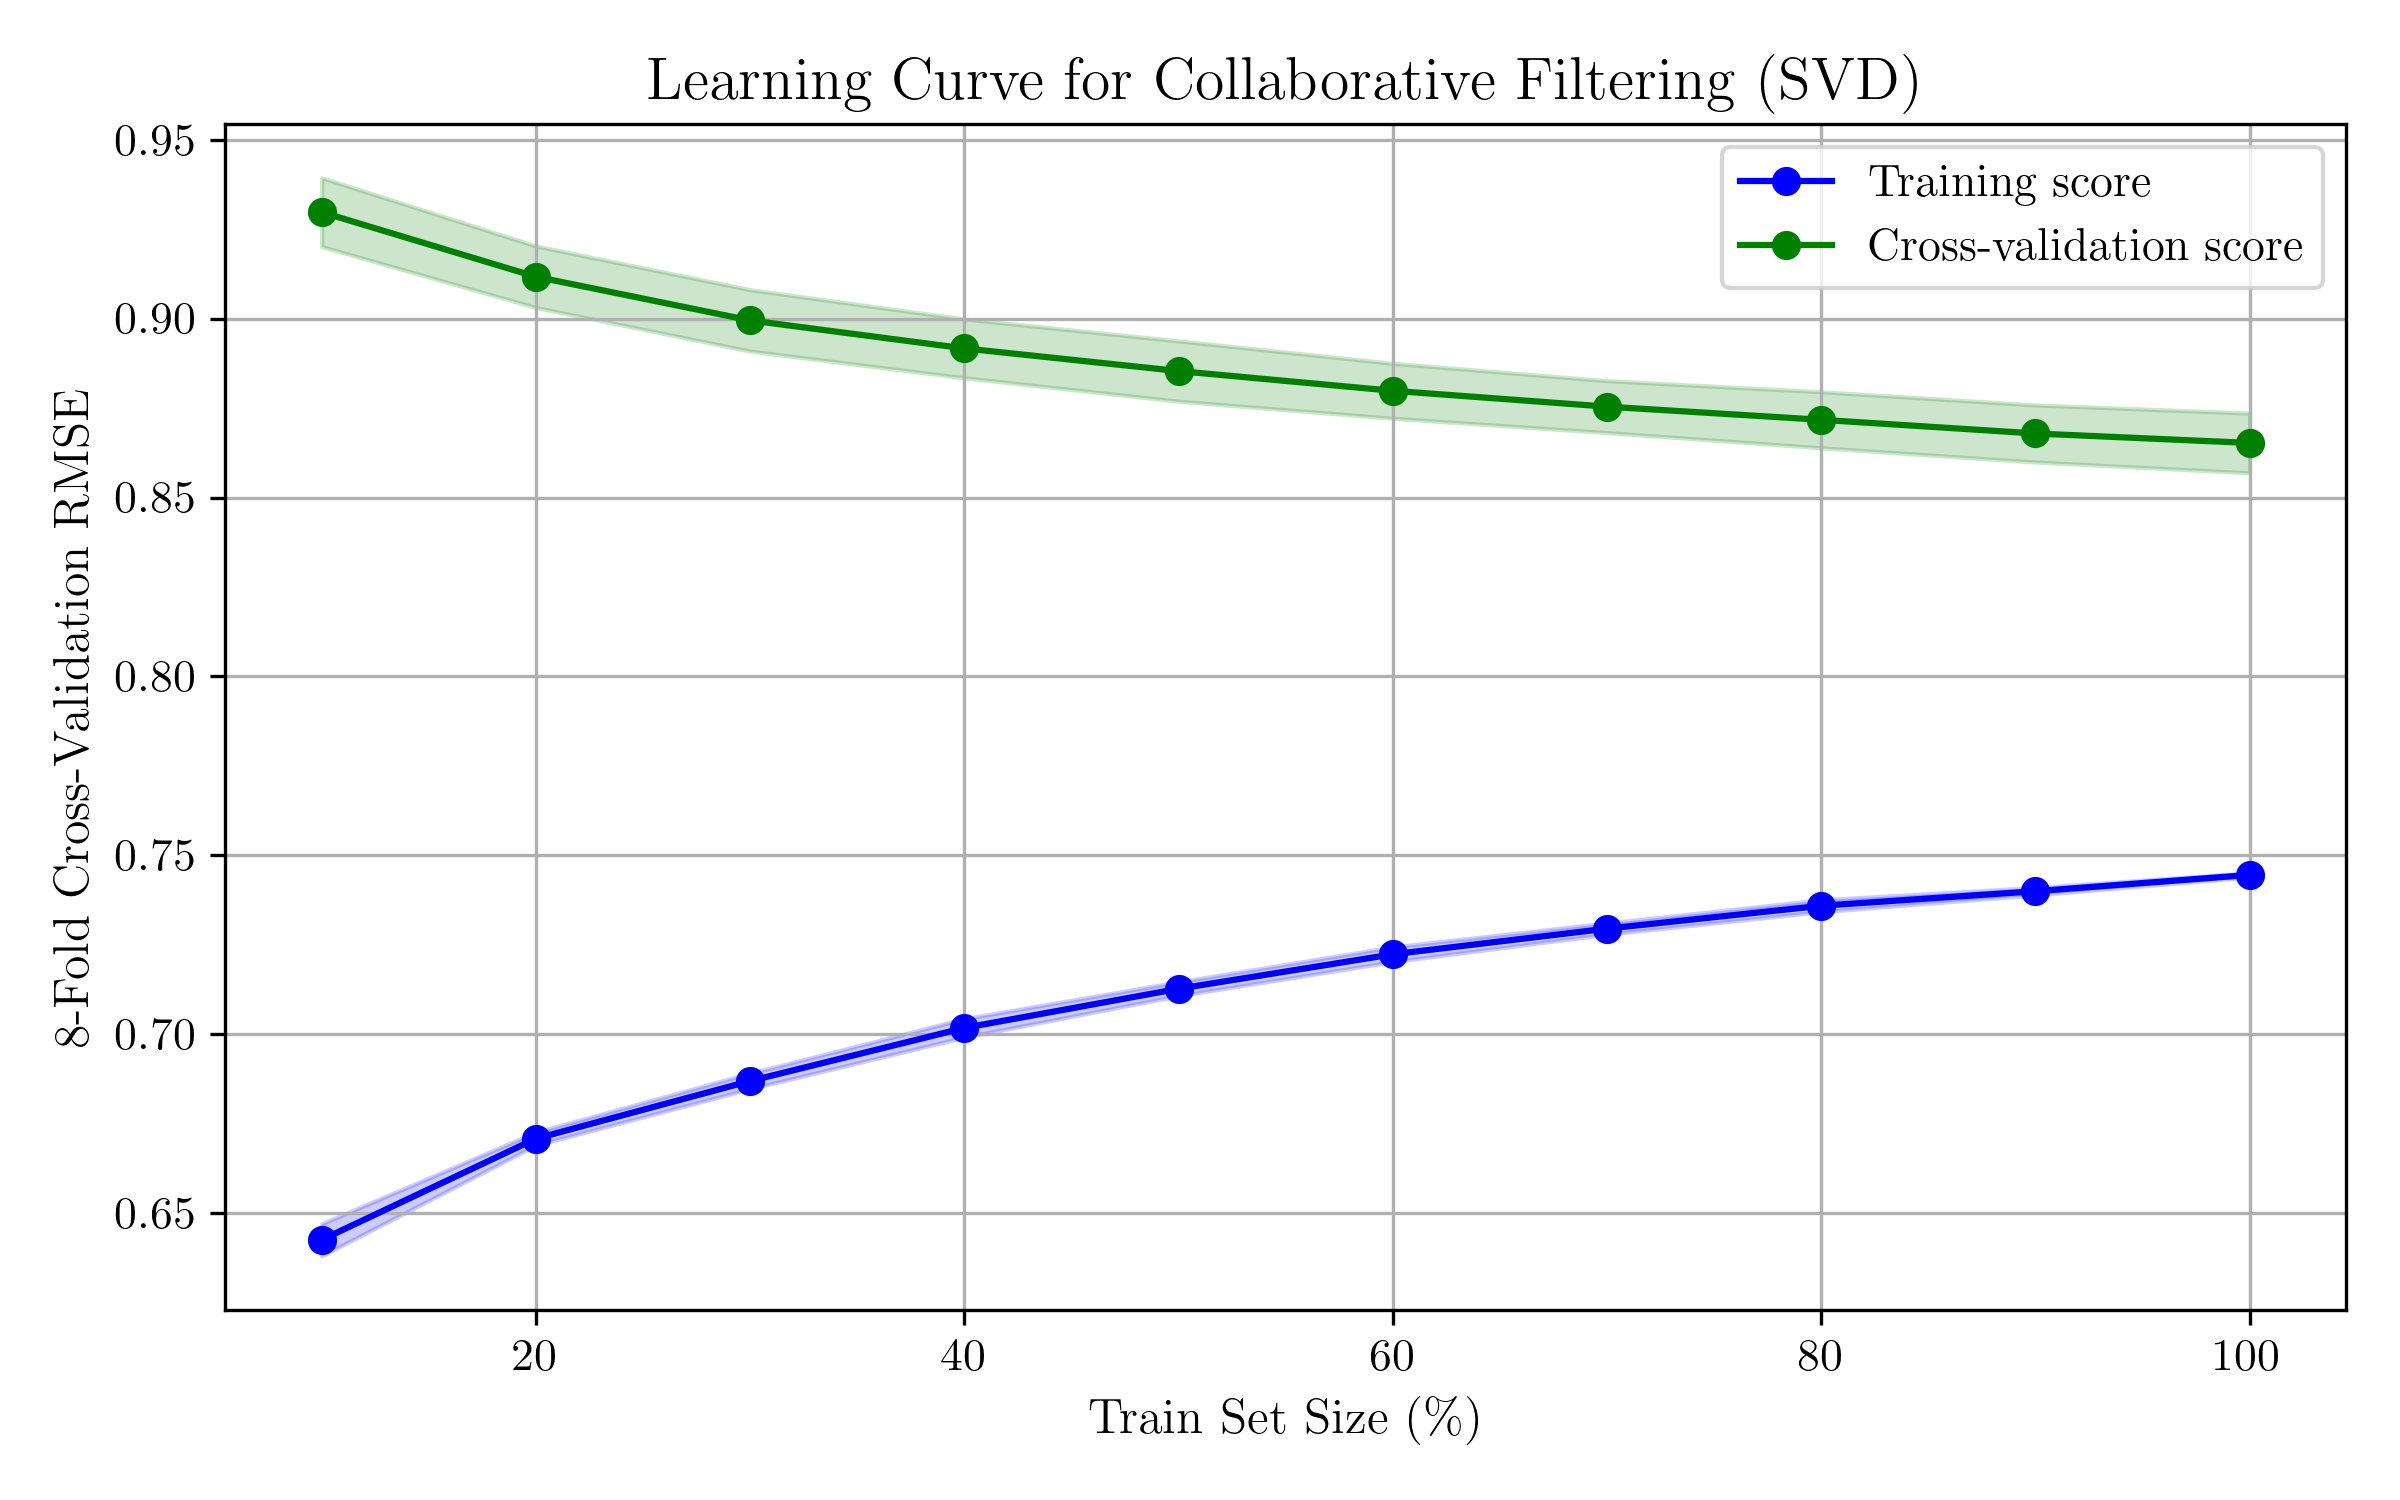
\includegraphics[width=1\linewidth]{assets/model03_learningcurve.png}
    \caption{CF-FunkSVD learning curve: 8-fold CV RMSE progression throughout the training dataset.}
    \label{fig:model03_learningcurve}
\end{figure}

As before, the error metrics evidence an adequate fit between the training and testing set, considering that there is not a significant increase of the error metrics between the training and the testing sets.
\newline
\newline
\begin{table}[H]
\centering
\caption{Error metrics for the train and test set (CF-FunkSVD), along with the number of samples for each.}
\label{tab:model03_results}
\begin{tabular}{lccc}
\toprule
\textbf{Dataset} & \textbf{RMSE} & \textbf{MAE} & \textbf{Support} \\
\midrule
Train Set & 0.75035 & 0.58313 & 80668 \\
Test Set & 0.87412 & 0.66957 & 20168 \\
\bottomrule
\end{tabular}
\end{table}


\section{Discussion} 
\subsection{Performance Metrics}

In order to assess the three models, RMSE and MAE are presented in the form of boxplot (Fig. \ref{fig:results_boxplot}, obtained by applying 8-fold CV to the whole dataset (7 folds for fitting and 1 fold for test), while using the optimized models. Despite the narrow range of errors, showing a high precision and repeatability for each model, CF-FunkSVD clearly outperforms both models for both error metrics.

\begin{figure}[H]
    \centering
    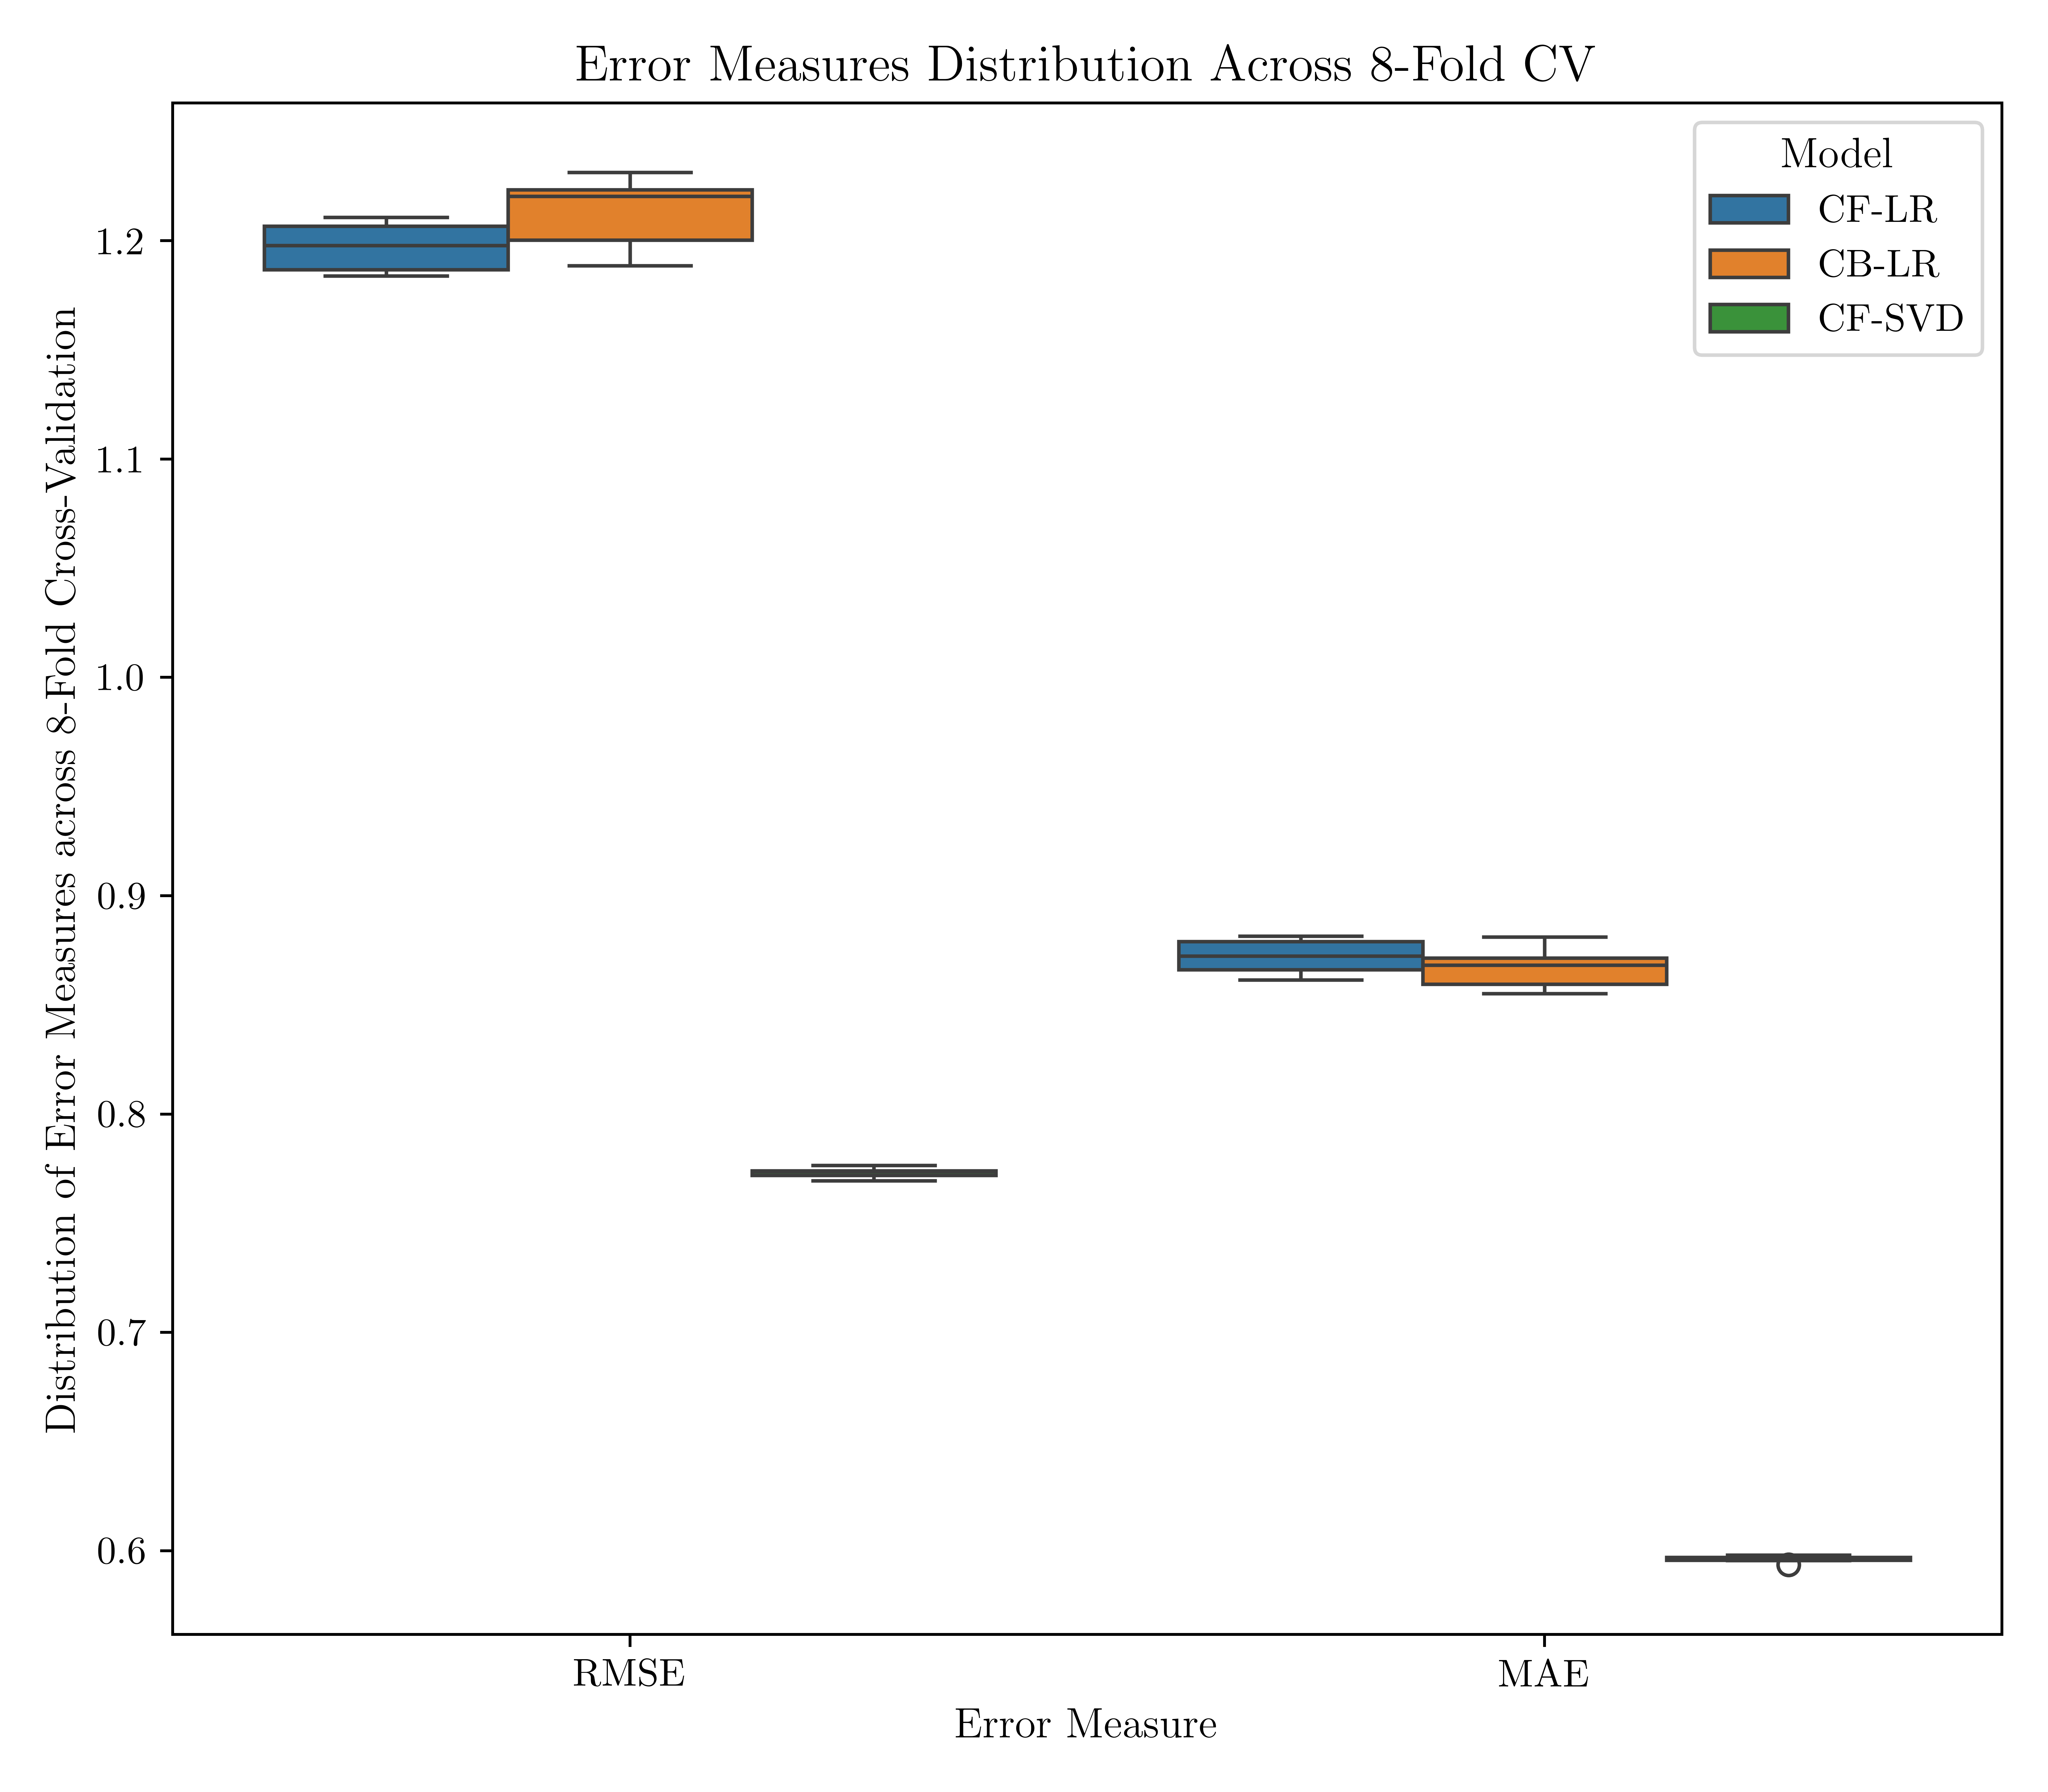
\includegraphics[width=1\linewidth]{assets/results_boxplot.png}
    \caption{Boxplot of RMSE and MAE error metrics determined by 8-fold CV across whole dataset.}
    \label{fig:results_boxplot}
\end{figure}

In Fig. \ref{fig:results_precisionK} to \ref{fig:results_mrrK}, Top-N metrics are used, presenting the performance of each model in the test set. These metrics intend to express the relevance of the items retrieved or the order in which these items are presented in a recommendation list. The metrics used were precision (proportion of retrieved items that are relevant), recall (proportion of relevant items that are retrieved), F1-score (weighted harmonic mean between precision and recall) and mean reciprocal rank (evaluates the position in which the first relevant item appears) \cite{9379914, ekstrand2020lenskit}.

\begin{align}
&\text{Precision@}k = \frac{|L \cap I_u|}{|L|} \notag \\
&\text{Recall@}k = \frac{|L \cap I_u|}{|I_u|} \notag \\
&\text{F1@}k = \frac{2 \times \text{Precision@}k \times \text{Recall@}k}{\text{Precision@}k + \text{Recall@}k} \notag \\
&\text{MRR} = \frac{1}{U} \sum_{u=1}^{U} \frac{1}{\text{rank}_u}
\end{align}

The value of these metrics depends on both the length of the suggestion lists, which in this analysis were computed for $k \in [10,100]$, and the reference list used for comparison ($I_u$), which was fixed to the Top-10 movies per user.

One thing to consider right from the beginning, is that the larger the list of ranked items the harder it is for any of the algorithms to accurately identify it. In most of the metrics, CF-FunkSVD performs better than the remaining, but only slightly better for the Top-100 items.


\begin{figure}[H]
    \centering
    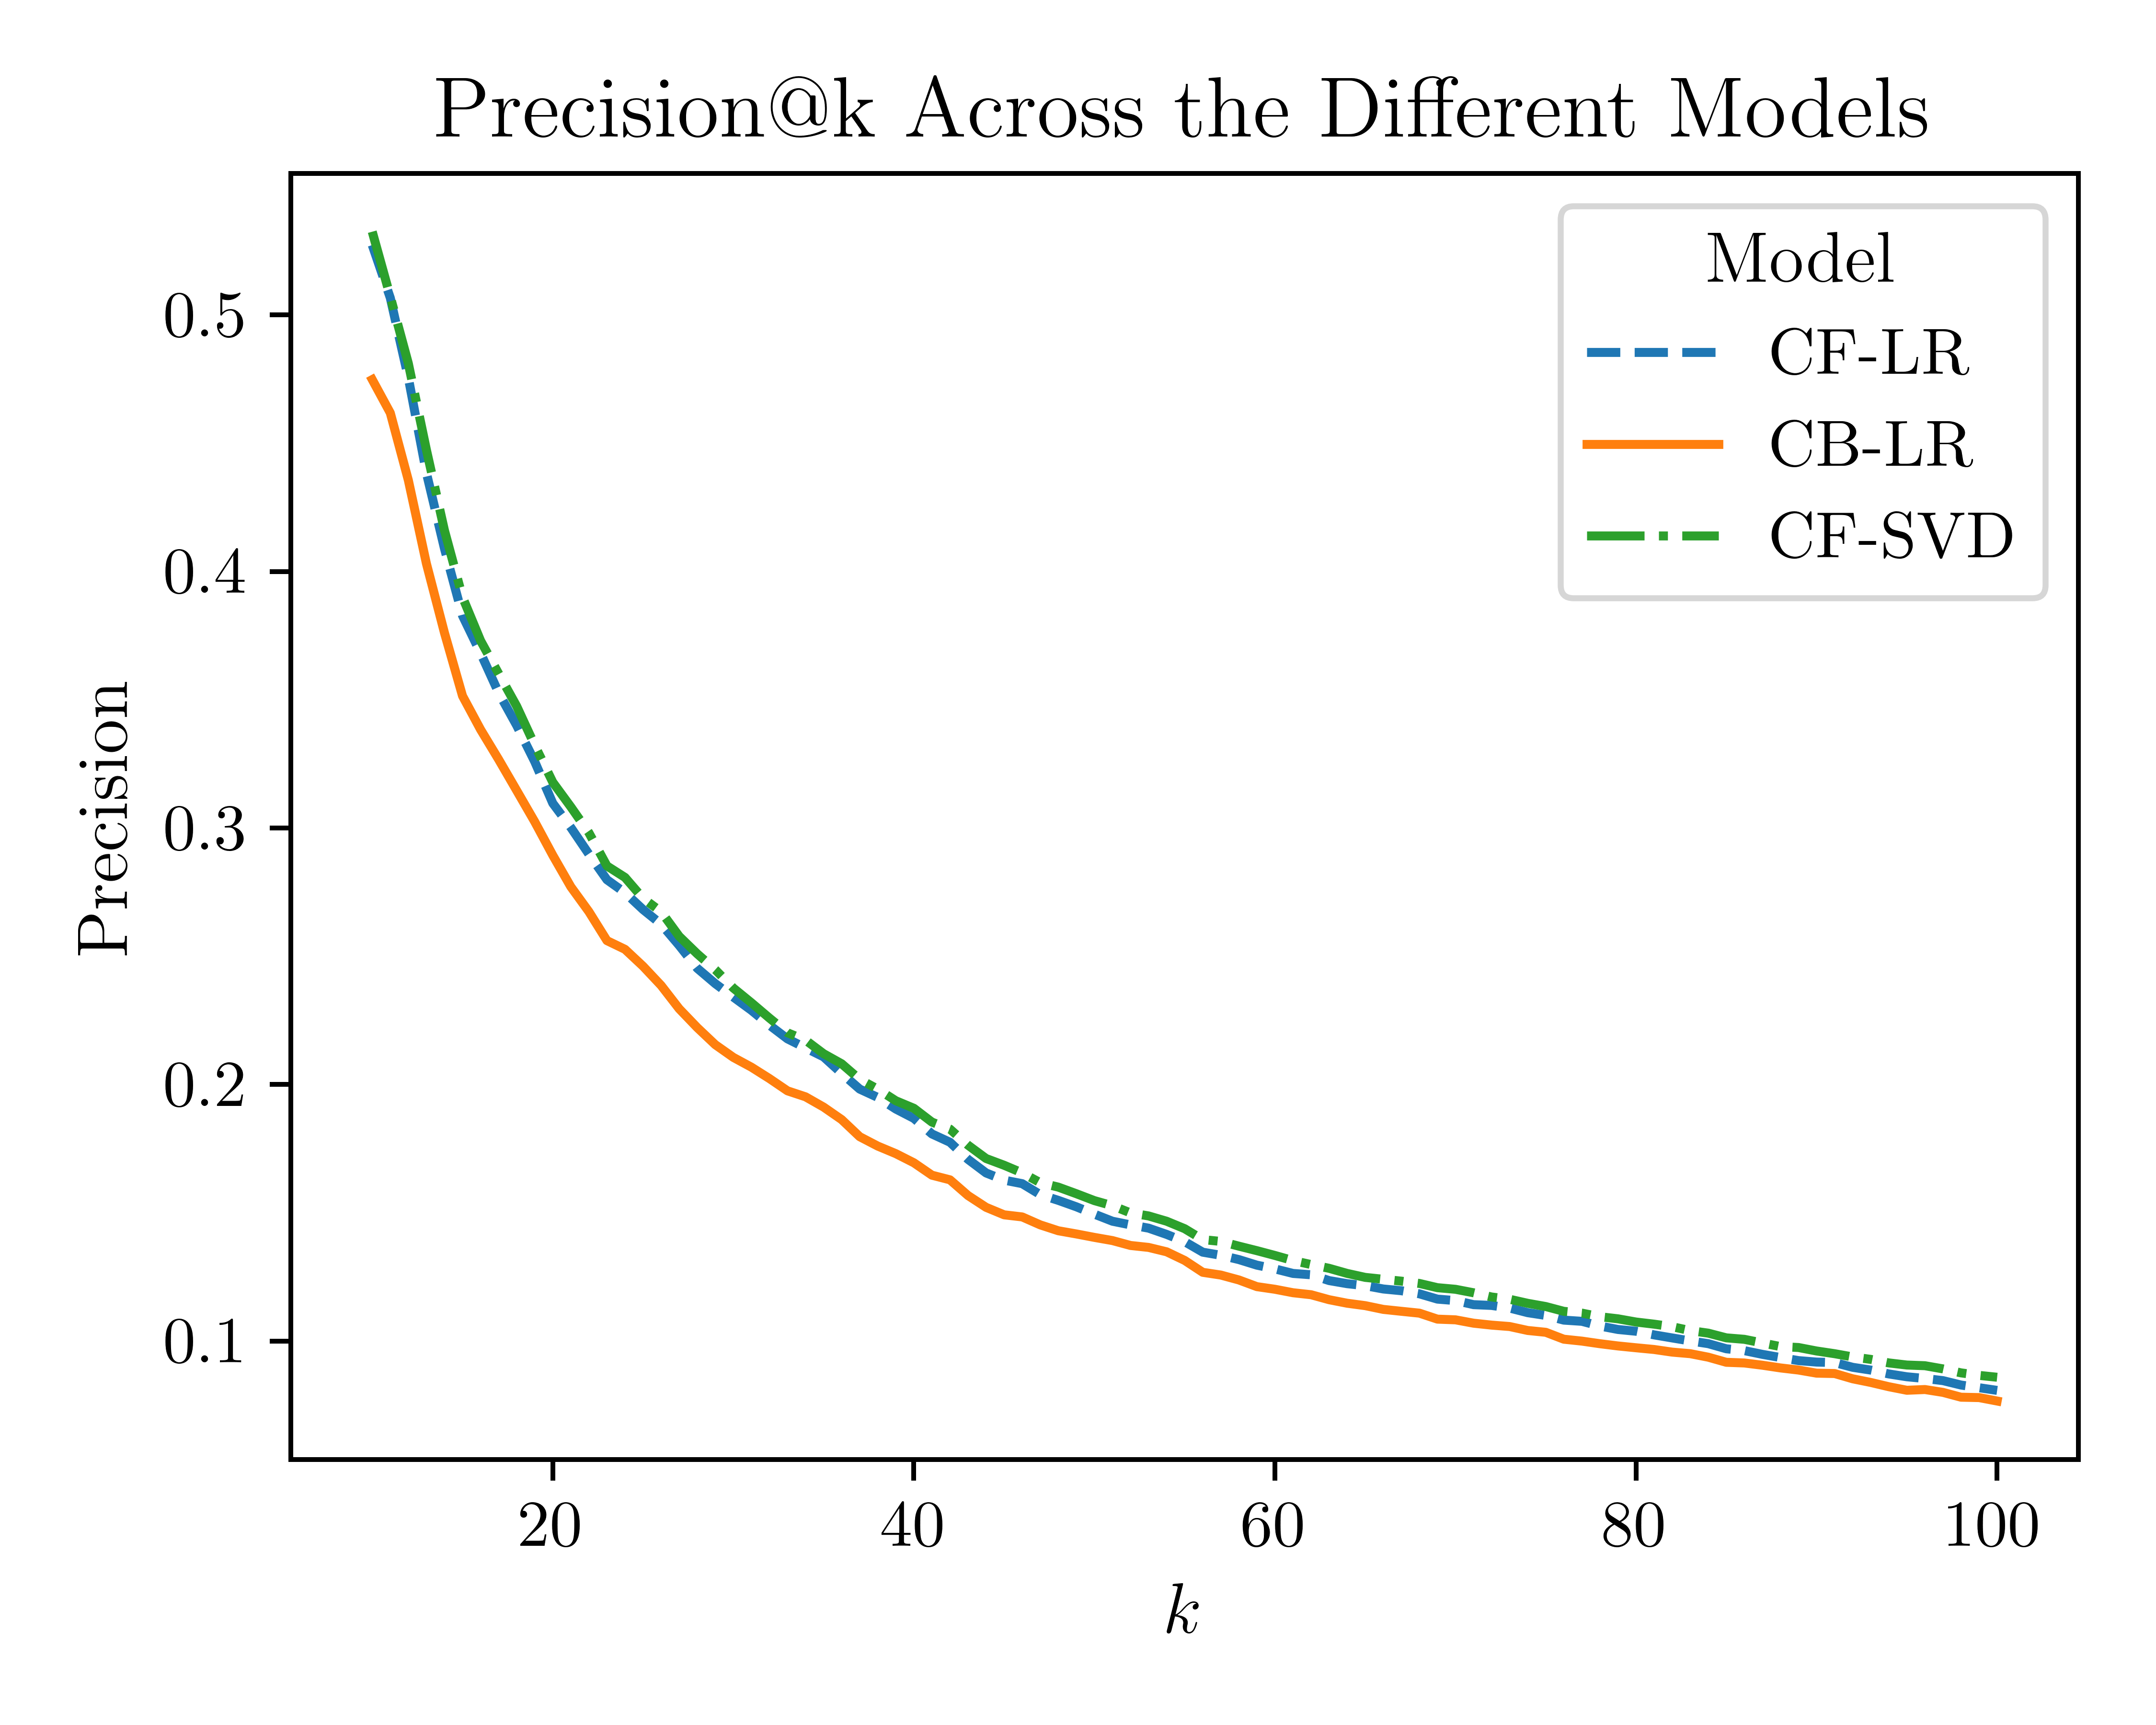
\includegraphics[width=1\linewidth]{assets/results_precisionK.png}
    \caption{Precision@$k$ for the test set, with $k \in [10,100]$ for the three models.}
    \label{fig:results_precisionK}
\end{figure}

Considering how recall is calculated (in relation to the relevance list per user), it is considerably better for CF-FunkSVD across the \textit{k} range, while F1@k is consistently better than the other two models. The CB-LR model performs well, considering its simplicity, suffering mostly due to the large error evidenced. 

For MRR, it is notable how CB-LR performs considerably worse than the other models (for any \textit{k}), considering that the features for the movies are estimated from their genres, indicating that this might be a good starting point, but needs refinement. Interestingly, the Top-100 ($k=100$) CF-LR surfaces as the best performing model, even though the performance over the whole range is comparable to that of CF-FunkSVD.

\begin{figure}[H]
    \centering
    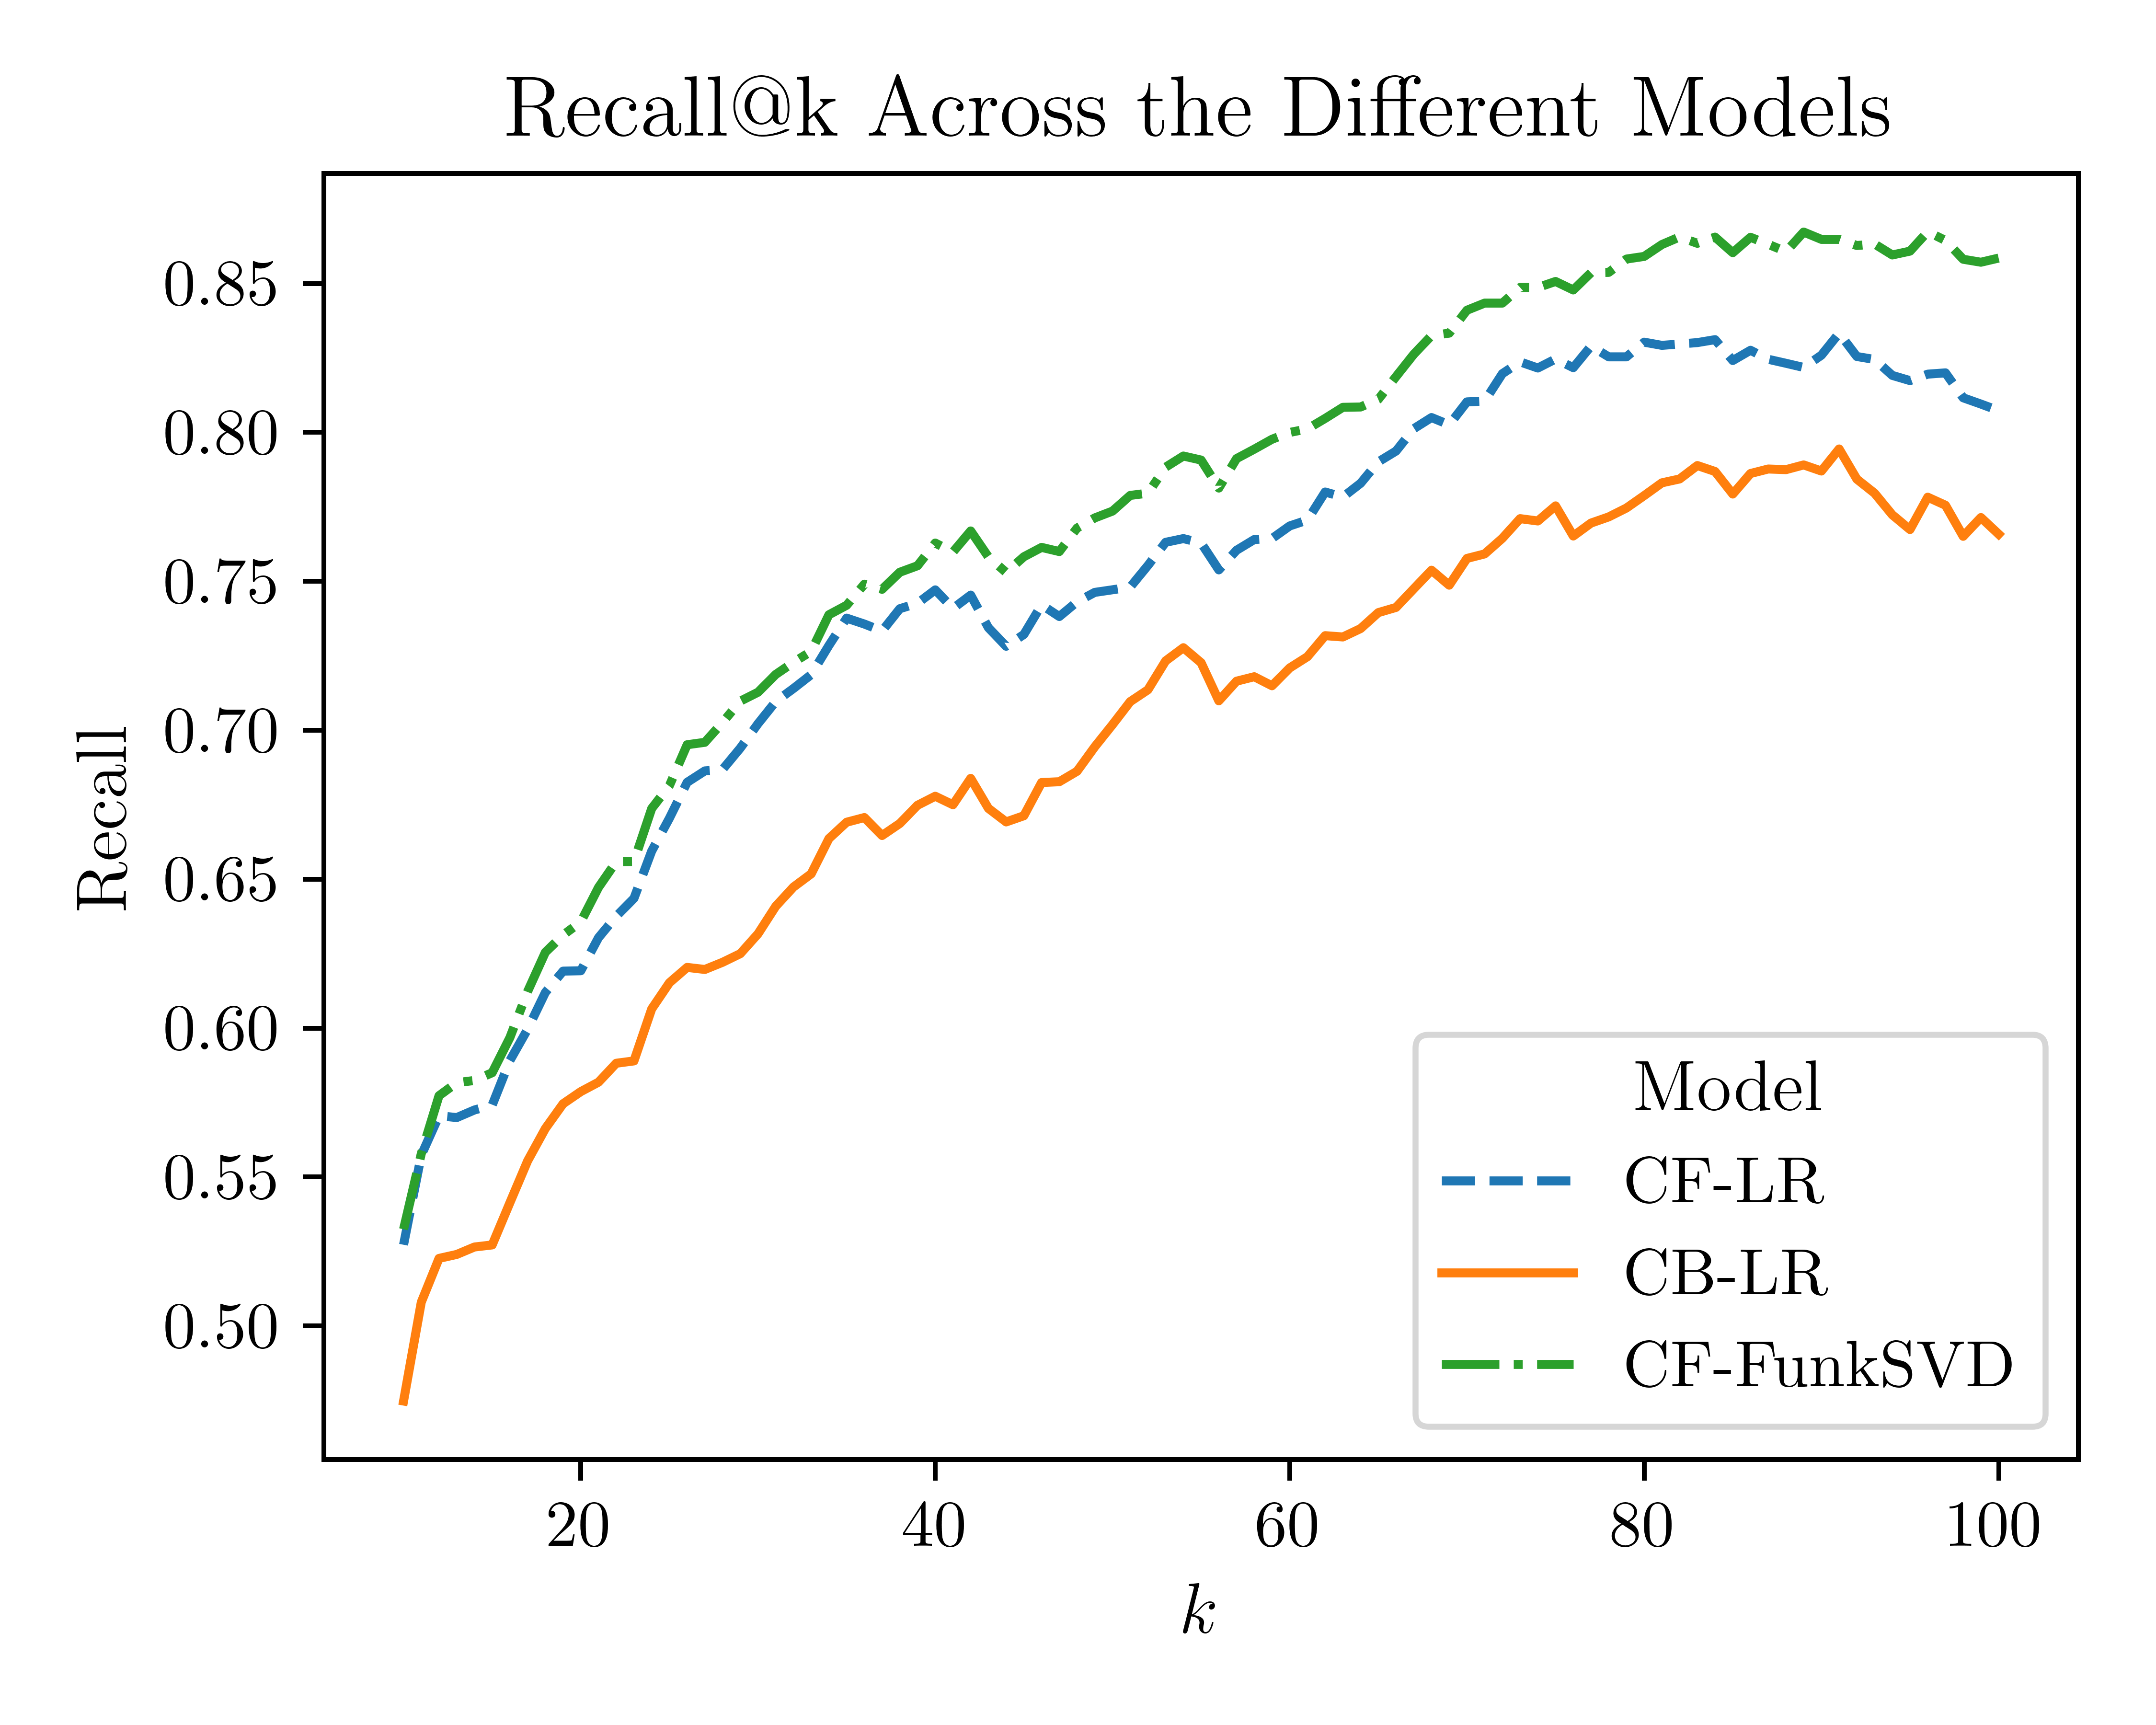
\includegraphics[width=1\linewidth]{assets/results_recallK.png}
    \caption{Recall@$k$ for the test set, with $k \in [10,100]$ for the three models.}
    \label{fig:results_recallK}
\end{figure}

\begin{figure}[H]
    \centering
    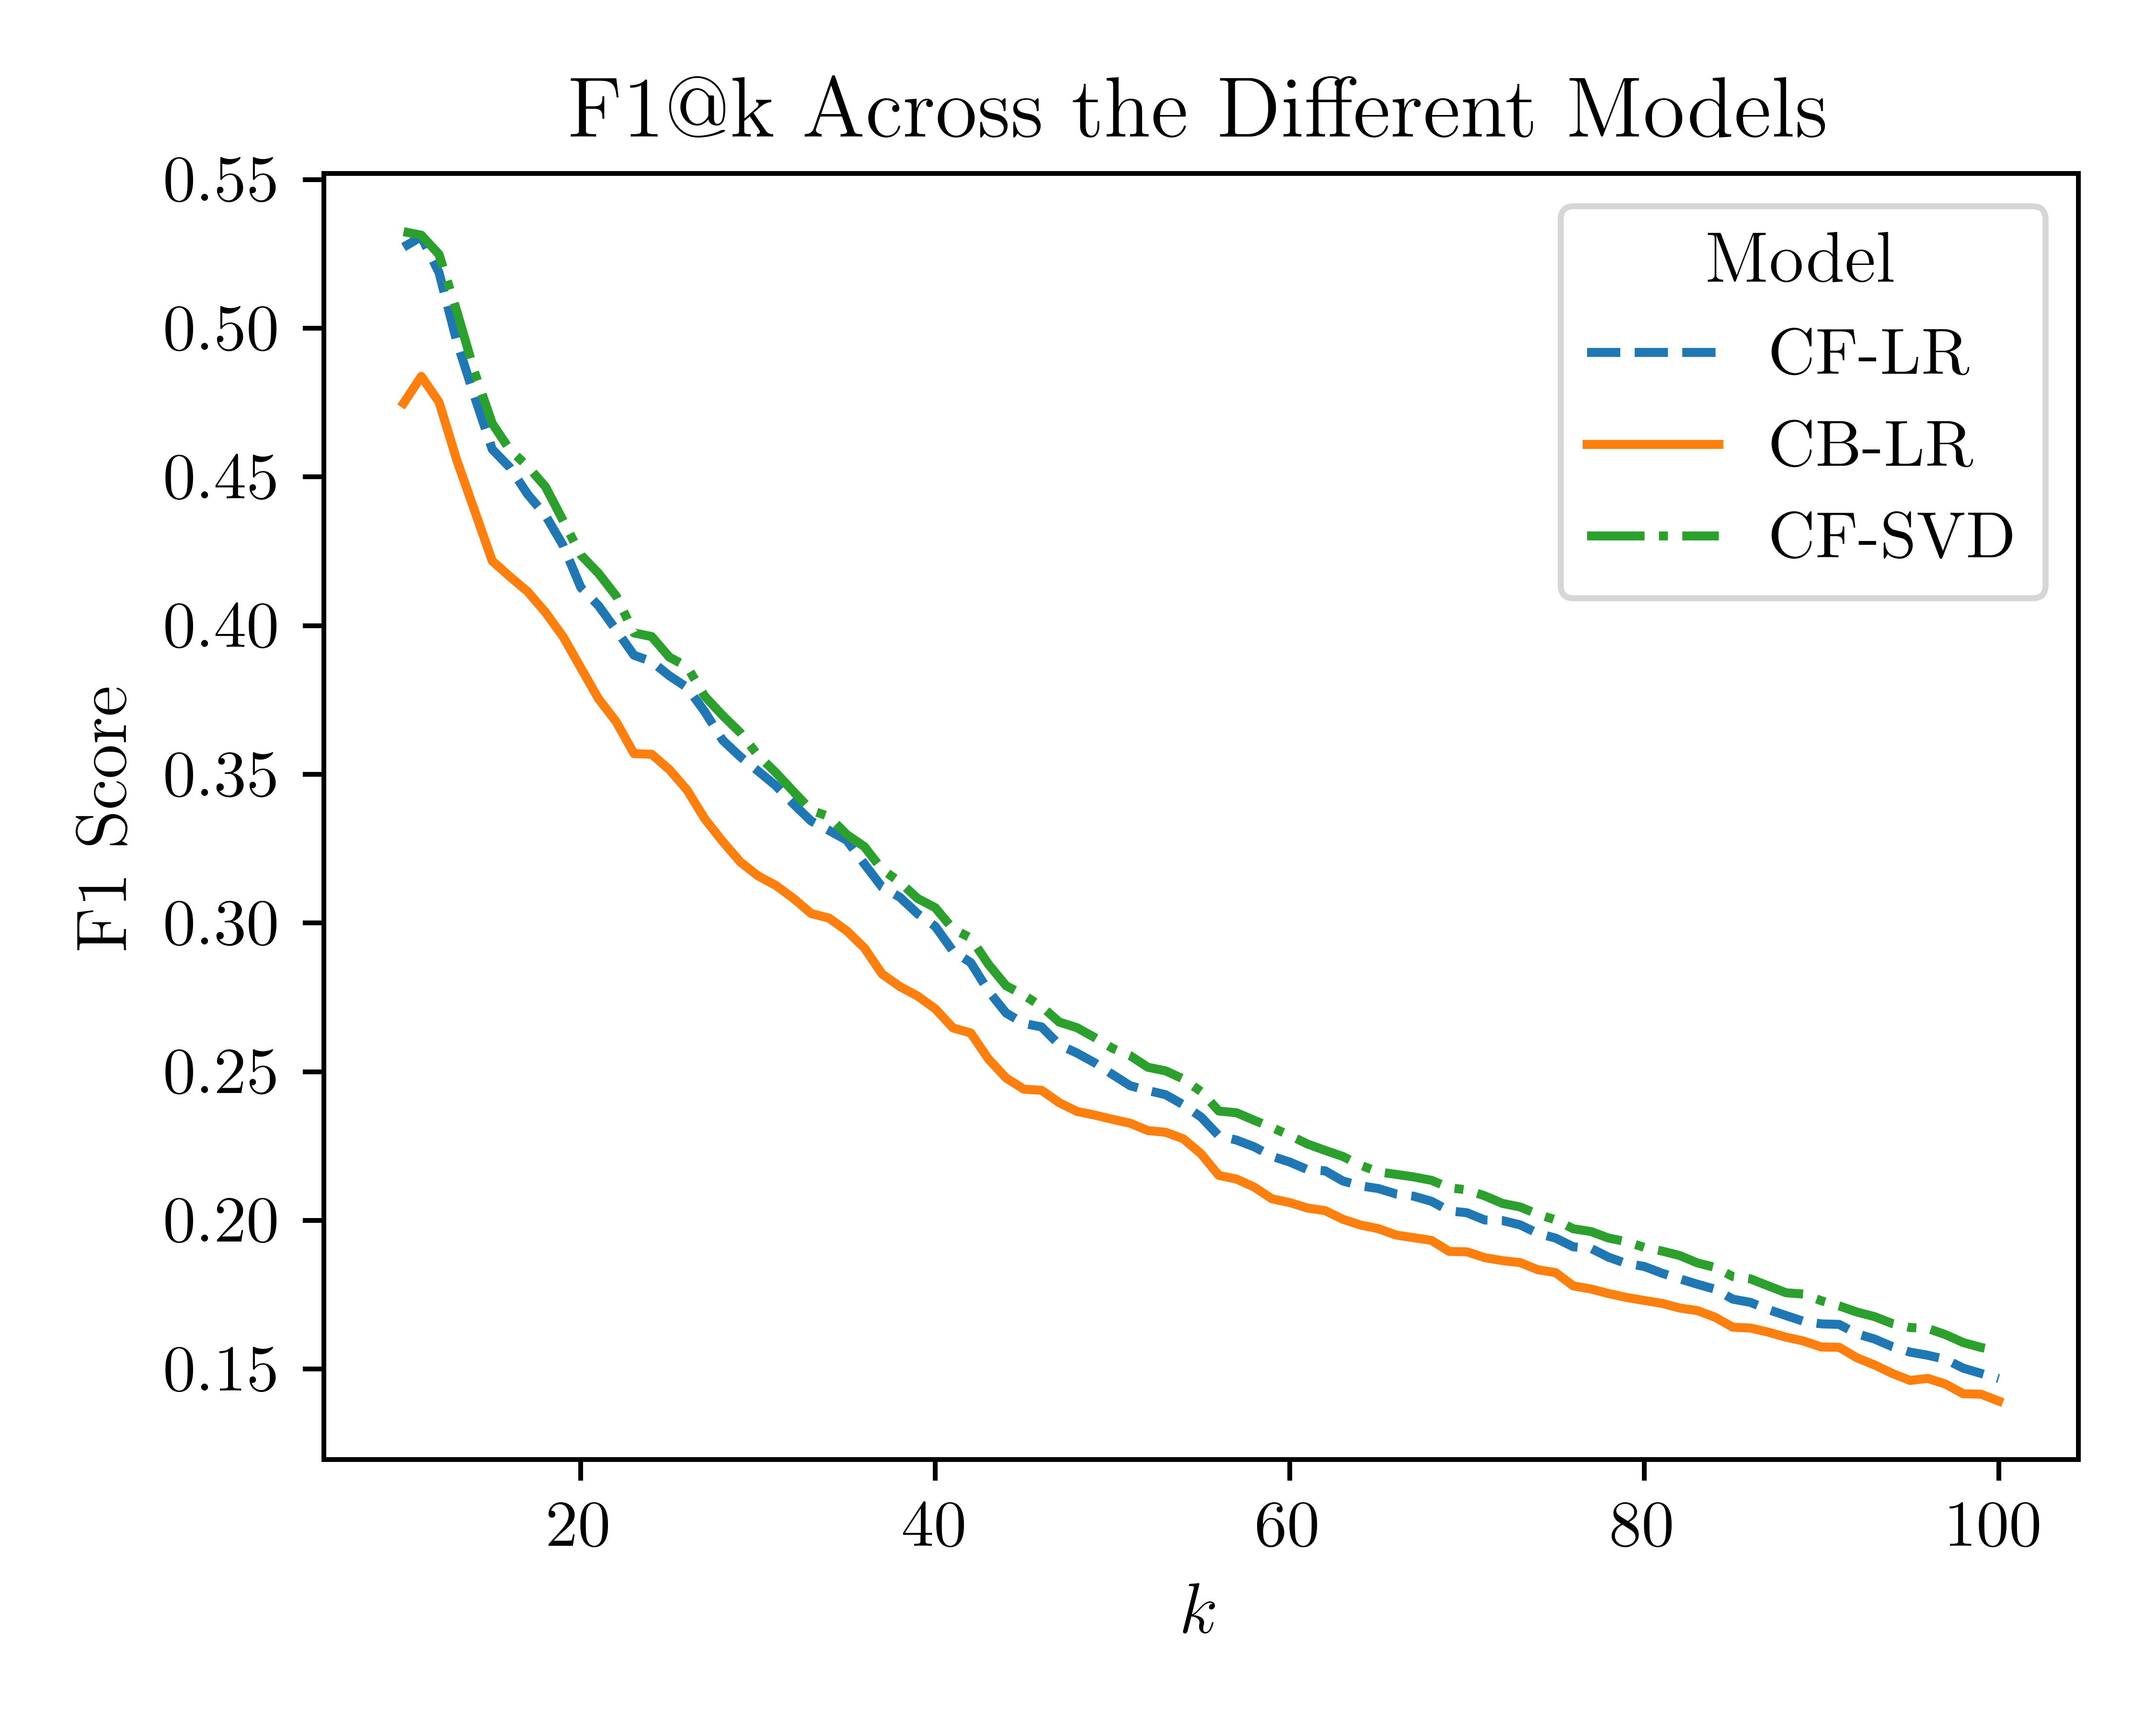
\includegraphics[width=1\linewidth]{assets/results_f1K.png}
    \caption{F1@$k$ for the test set, with $k \in [10,100]$ for the three models.}
    \label{fig:results_f1K}
\end{figure}

\begin{figure}[H]
    \centering
    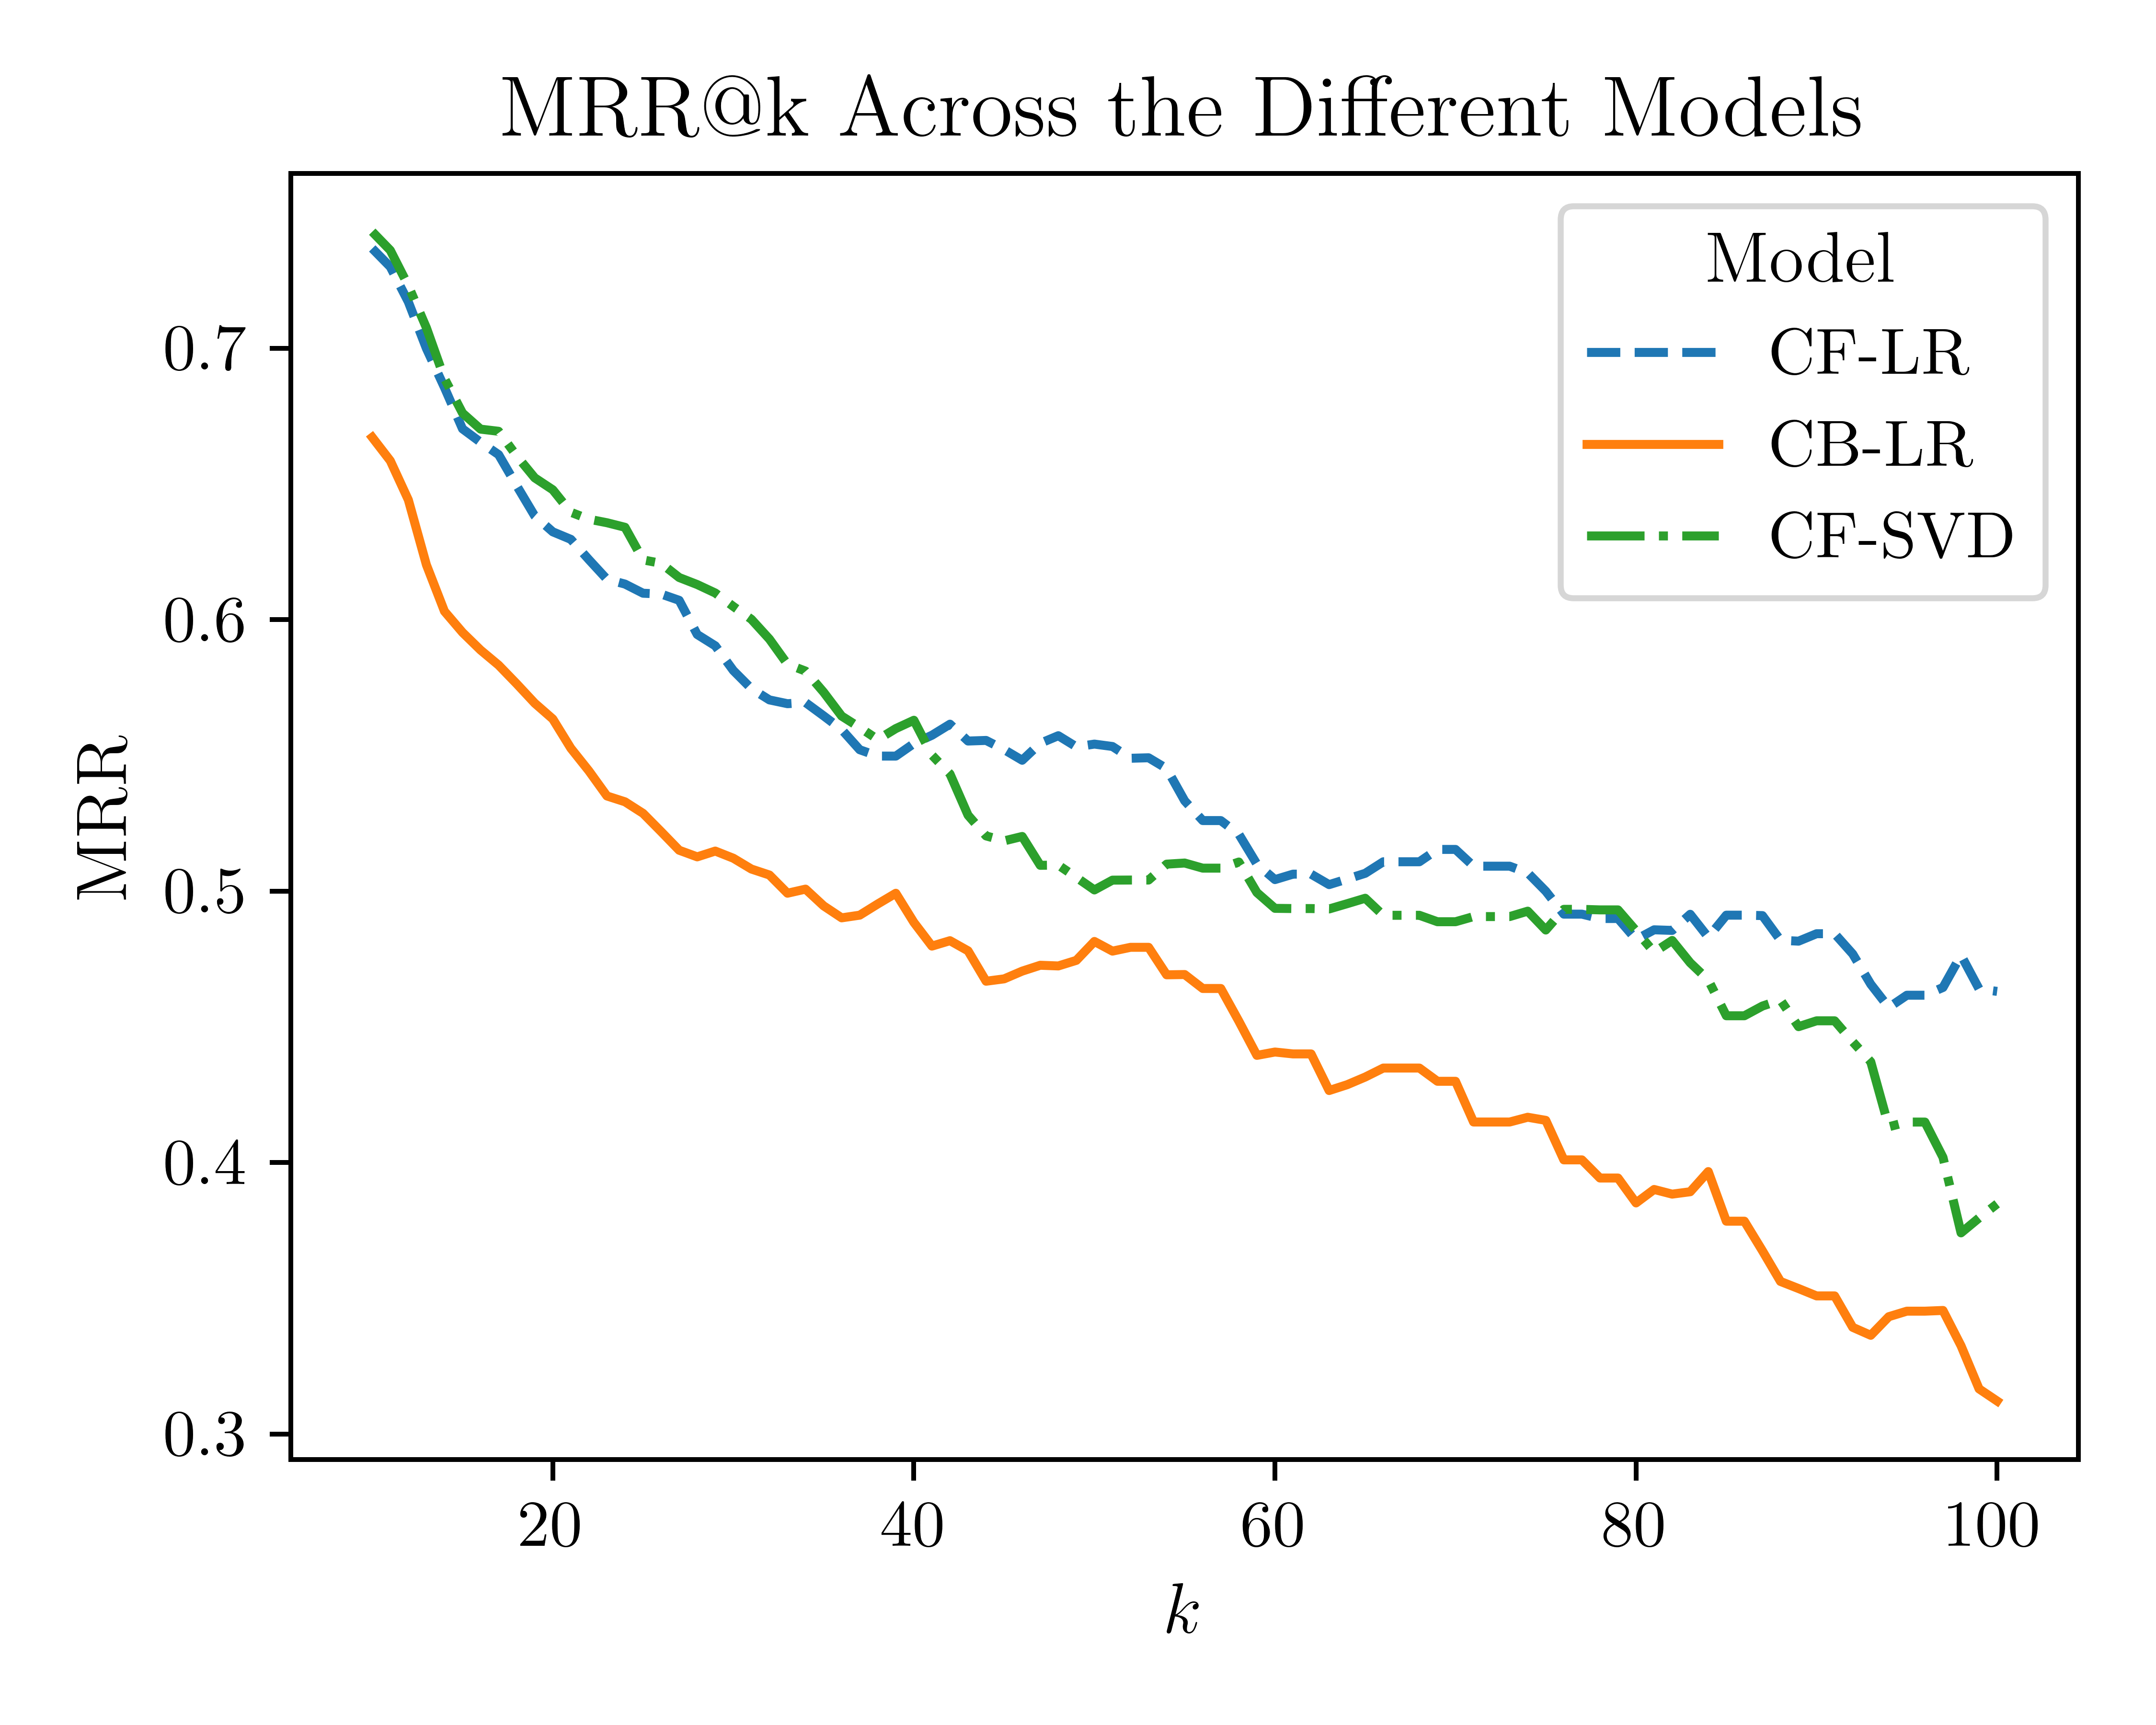
\includegraphics[width=1\linewidth]{assets/results_mrrK.png}
    \caption{MRR@$k$ for the test set, with $k \in [10,100]$ for the three models.}
    \label{fig:results_mrrK}
\end{figure}

\subsection{Literature Benchmark}

The models in question are simpler in application compared to CF-FunkSVD, however, it is worthwhile to reflect on their performance comparing with the literature. First and foremost, the differences at this level are not so significant, as the CF-FunkSVD depends largely on fine tuning of the multitude of hyperparameters available. Nonetheless, it still outperforms both types of linear regression.

\begin{table}[H]
\centering
\caption{Models performance results for the test set.}
\label{tab:atk_results_benchamarkpaper}
\begin{tabular}{lccc}
\toprule
\textbf{Measure} & \textbf{CF-LR} & \textbf{CB-LR} & \textbf{CF-FunkSVD} \\
\midrule
Precision@100 & 0.08073 & 0.07659 & 0.08585 \\
Recall@100 & 0.80732 & 0.76585 & 0.85854 \\
F1@100 & 0.14679 & 0.13925 & 0.15610 \\
MRR@100 & 0.46304 & 0.31212 & 0.38477 \\
RMSE & 1.23691 & 0.97240 & 0.87268 \\
MAE & 0.90417 & 0.74607 & 0.66804 \\
\bottomrule
\end{tabular}
\end{table}

In the study conducted by Paullier et al. \cite{9379914}, seven different models were tested under identical conditions, offering a comprehensive comparison framework and approach to addressing this type of problem. The models developed and presented in this paper align well with the performance benchmarks reported in the literature.

While Table \ref{tab:atk_results_benchamarkpaper} closely resembles the results presented in Paullier’s work, it is important to note that the datasets used are different. Paullier et al. utilized the smaller MovieLens 100k dataset, whereas the current work is based on a larger dataset, allowing for a more robust application of the FunkSVD algorithm. This distinction highlights an improvement in performance metrics for the FunkSVD model developed in this paper, driven by the larger dataset’s ability to better capture and fit the algorithm's underlying structure.

\section{Conclusion}

The purpose of this project was to learn, assess, and employ different recommendation systems. The literature review allowed to understand how different models based on collaborative filtering emerged throughout the years, and one of the biggest motivations for the rapid expansion of the field, the Netflix prize. The dataset used is a benchmark in this type of studies, decently sized, which allowed for proper fitting of the models and comparison with the literature.

The developed models offer opportunities for further enhancement. Both collaborative filtering (CF-LR) and content-based (CB-LR) models could benefit from a more systematic approach to determining the optimal number of features, rather than relying on empirical estimates. Additionally, the third model presents numerous hyperparameters that warrant fine-tuning, which could serve as a dedicated research endeavor. There are several promising directions for future exploration, including incorporating the FunkSVD model into an ensemble algorithm.


\section*{Work Load}

Both authors contributed equally to the project.

\bibliographystyle{IEEEtran}
\bibliography{references}

\end{document}



